













\twocolumn[{%
\renewcommand\twocolumn[1][]{#1}%
{\Huge \textbf{Appendix}}
\vspace{-0.6cm}
\begin{center}
	\vspace{0.5cm}
    \captionsetup{type=figure}
    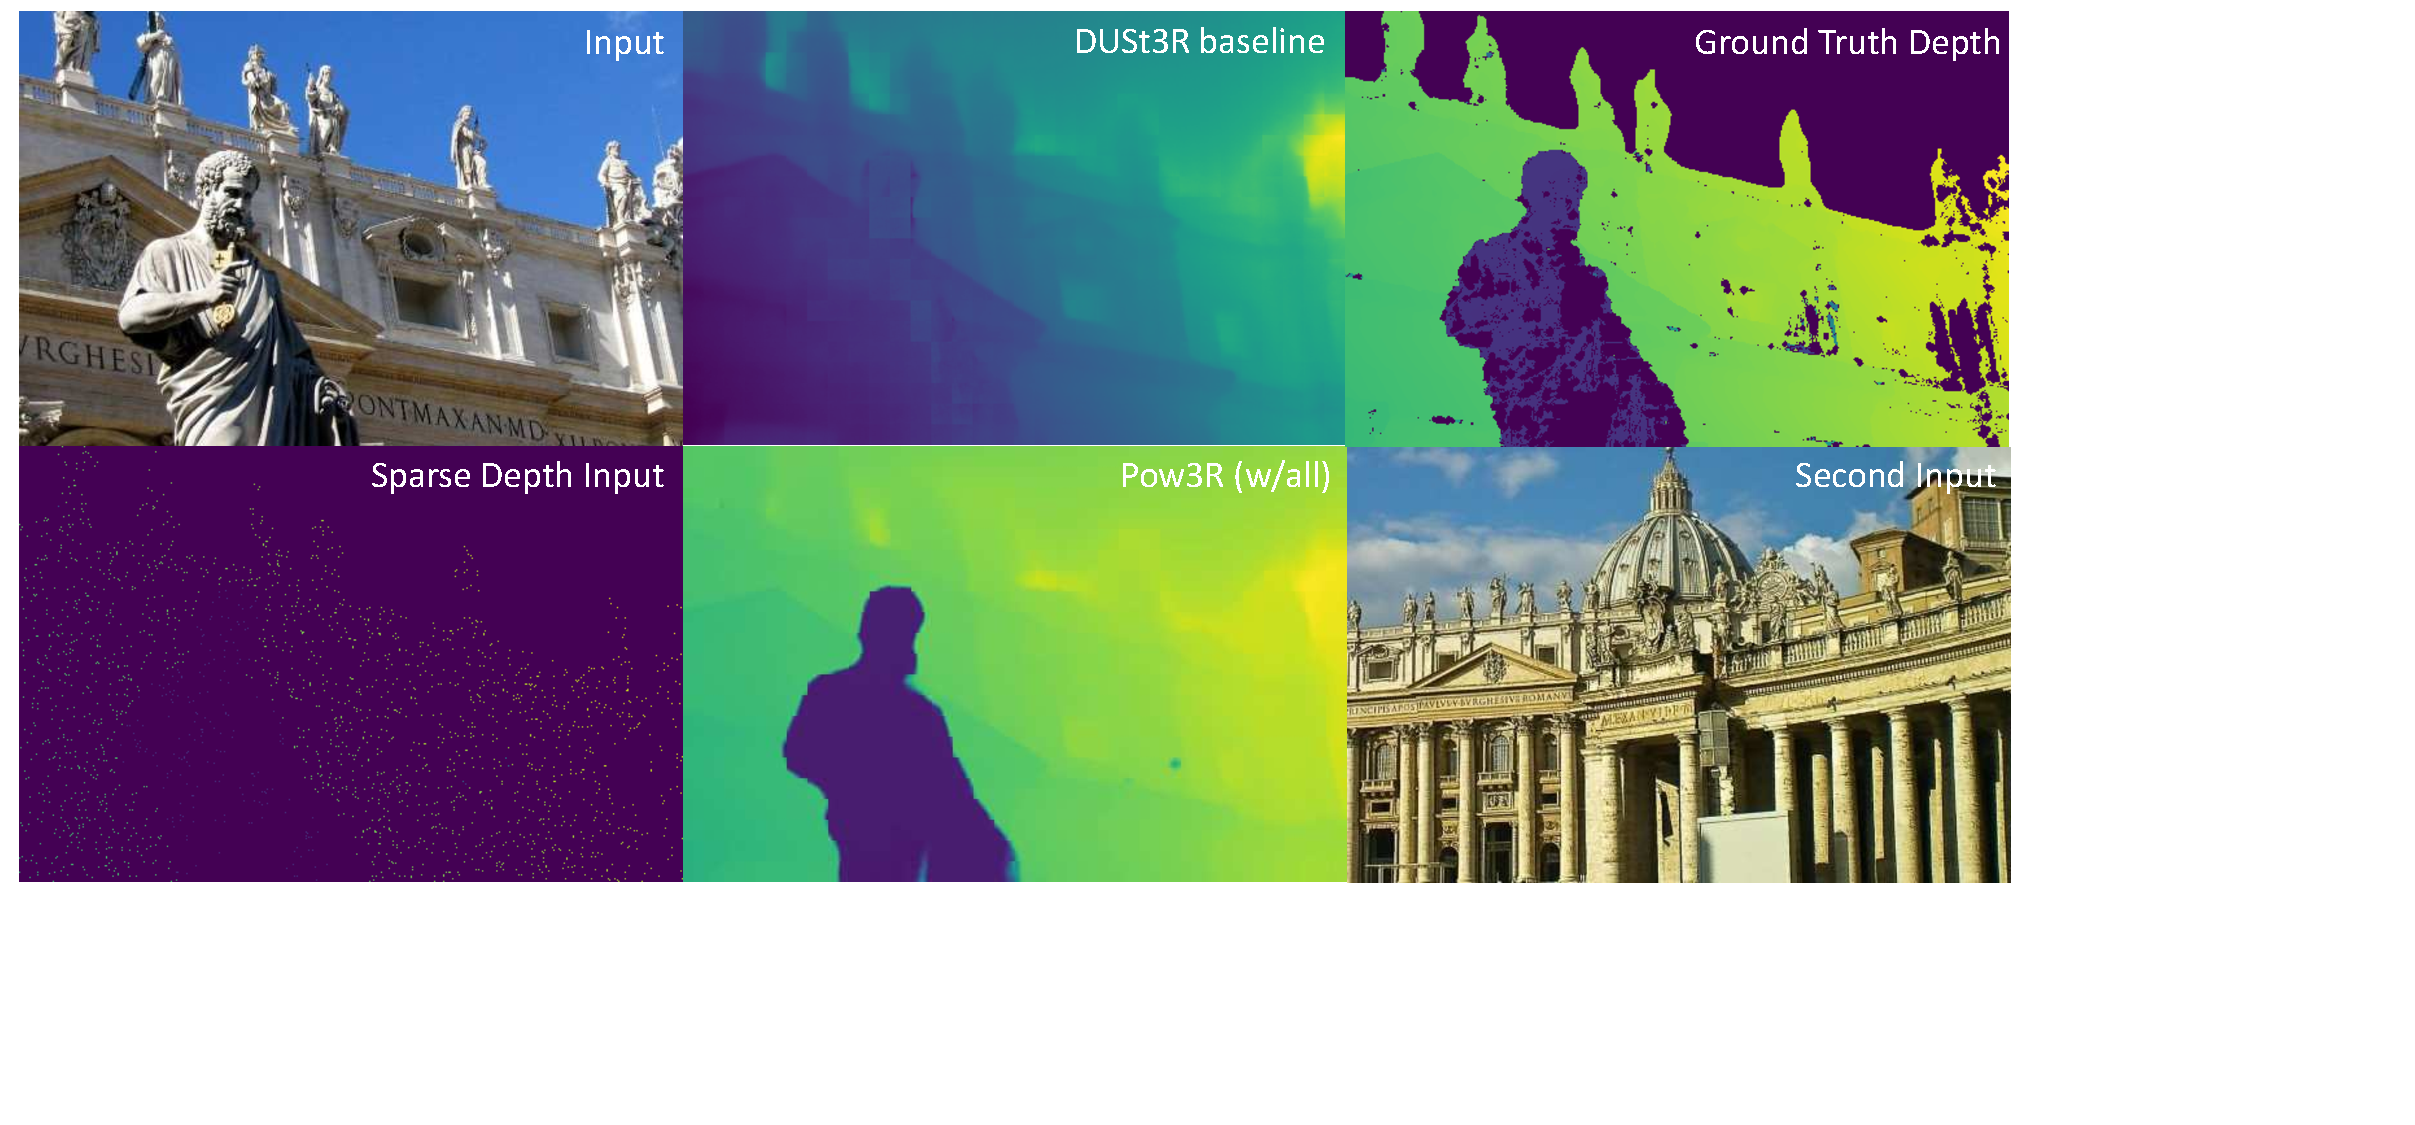
\includegraphics[width=\linewidth,trim=0 115 195 0,clip]{figures/supp/megadepth-statue.pdf}
    \vspace{-0.65cm}
    \captionof{figure}{\textbf{Qualitative Result in terms of predicted depthmaps.} We compare \ours{} with \duster{} on one of the Megadepth~\cite{li2018megadepth} outdoor scenes (from the validation set). For this evaluation, we feed camera intrinsics, pose as well as 2048 sparse point clouds. The figure clearly demonstrates that \duster{} fails to accurately  capture the statue, while \ours{} reconstructs it correctly.}
    \label{fig:qualitative_megadepth_statue}
\end{center}
}]


\section{Further Experiments on the Impact of Guiding}

In Table 1 of the main paper, we perform experiments on the Habitat validation dataset to study the impact of each auxiliary modality on the reconstruction accuracy in terms of different metrics. 
In Table~\ref{tab:modality_study_infinigen}, we perform the same experiment on data generated with Infinigen~\cite{Raistrick2023Infinigen}. 
Compared to Habitat, InfiniGen offers two advantages: 
(i) InfiniGen is free of artifacts, which can be numerous in the Habitat dataset due to acquisition problem on windows, mirrors, complex surfaces, \etc;
(ii) there is no risk of training data contamination or overfitting, as InfiniGen is not part of the training set at all.
Nevertheless, we observe similar results and trends than on Habitat, highlighting the robustness of these findings.

\begin{table}[]
    \centering
    \definecolor{darkgreen}{HTML}{005701}
    \newcommand{\withmod}{\checkmark}
    \newcommand{\withoutmod}{$\times$}
    \newcommand{\firstcell}[1]{#1 & }
    \newcommand{\onediffcell}[2]{#1 & \textcolor{darkgreen}{\small (+#2)}}
    \resizebox{\linewidth}{!}{
    \begin{tabular}{c|c@{~~}c@{~~}c@{~~}c@{~~}c|r@{}rr@{}rr@{}rr@{}r}
    \toprule
     & \multicolumn{5}{c|}{aux. modalities} & \multicolumn{2}{c}{focal} & \multicolumn{2}{c}{depth} & \multicolumn{4}{c}{rel. pose} \\
     & K1 & K2 & D1 & D2 & RT & \multicolumn{2}{c}{acc@1.015} & \multicolumn{2}{c}{$\tau$@1.03} & \multicolumn{2}{c}{RRA@2$^\circ$} & \multicolumn{2}{c}{RTA@2$^\circ$} \\
    \midrule
    
    DUSt3R & \withoutmod & \withoutmod & \withoutmod & \withoutmod & \withoutmod & \firstcell{28.4} & \firstcell{75.9} & \firstcell{64.6} & \firstcell{27.2} \\
    \midrule
    {\textbf{\ours{}}} & \withoutmod & \withoutmod & \withoutmod & \withoutmod & \withoutmod 
    & \firstcell{29.8} & \firstcell{75.1} & \firstcell{66.5} & \firstcell{30.4} \\
     & \withmod & \withoutmod & \withoutmod & \withoutmod & \withoutmod & \onediffcell{60.7}{30.9} & \onediffcell{75.5}{0.4} & \onediffcell{70.3}{3.8} & \onediffcell{35.2}{4.8} \\
     & \withoutmod & \withmod & \withoutmod & \withoutmod & \withoutmod & \onediffcell{60.5}{30.7} & \onediffcell{75.8}{0.7} & \onediffcell{70.9}{4.4} & \onediffcell{37.0}{6.6} \\
     & \withmod & \withmod & \withoutmod & \withoutmod & \withoutmod & \onediffcell{89.8}{60.0} & \onediffcell{76.2}{1.1} & \onediffcell{73.7}{7.2} & \onediffcell{50.0}{19.6} \\
     & \withoutmod & \withoutmod & \withmod & \withoutmod & \withoutmod & \onediffcell{34.3}{4.5} & \onediffcell{87.9}{12.8} & \onediffcell{70.9}{4.4} & \onediffcell{35.3}{4.9} \\
     & \withoutmod & \withoutmod & \withoutmod & \withmod & \withoutmod & \onediffcell{34.3}{4.5} & \onediffcell{88.3}{13.2} & \onediffcell{71.0}{4.5} & \onediffcell{35.3}{4.9} \\
     & \withoutmod & \withoutmod & \withmod & \withmod & \withoutmod & \onediffcell{40.9}{11.0} & \onediffcell{94.9}{19.8} & \onediffcell{74.6}{8.1} & \onediffcell{46.5}{16.1} \\
     & \withoutmod & \withoutmod & \withoutmod & \withoutmod & \withmod & \onediffcell{34.9}{5.1} & \onediffcell{76.0}{0.9} & \onediffcell{86.6}{20.1} & \onediffcell{54.3}{23.9} \\
     & \withmod & \withmod & \withmod & \withmod & \withoutmod & \onediffcell{98.0}{68.1} & \onediffcell{\textbf{95.4}}{\textbf{20.3}} & \onediffcell{82.2}{15.7} & \onediffcell{71.0}{40.6} \\
     & \withmod & \withmod & \withoutmod & \withoutmod & \withmod & \onediffcell{90.6}{60.8} & \onediffcell{77.0}{1.9} & \onediffcell{91.1}{24.7} & \onediffcell{72.2}{41.8} \\
     & \withoutmod & \withoutmod & \withmod & \withmod & \withmod & \onediffcell{50.2}{20.4} & \onediffcell{95.0}{19.9} & \onediffcell{93.0}{26.5} & \onediffcell{70.5}{40.1} \\
     & \withmod & \withmod & \withmod & \withmod & \withmod & \onediffcell{\textbf{98.5}}{\textbf{68.6}} & \onediffcell{\textbf{95.4}}{\textbf{20.3}} & \onediffcell{\textbf{97.4}}{\textbf{30.9}} & \onediffcell{\textbf{90.2}}{\textbf{59.8}} \\
    \bottomrule
        \end{tabular}
    }
    \vspace{-0.3cm}
    \caption{\textbf{Impact of guiding at test time} for models trained at $224{\times}224$ resolution. We report performances on InfiniGen for DUSt3R, which cannot handle auxiliary modalities, and our single model with different sets of modalities; we show in green the absolute improvement \wrt the results without auxiliary modality. 
    }
    \vspace{-0.2cm}
    \label{tab:modality_study_infinigen}
\end{table}





\section{Multi-View Depth Estimation results}

\begin{table*}
\begin{center}
\renewcommand\arraystretch{1.2}
\setlength{\tabcolsep}{1pt} 
\scriptsize 
\small
\hspace{-3mm}
\resizebox{\textwidth}{!}{
\begin{tabular}{llccccrrrrrrrrrrrrc}
 \hline
\specialrule{1.5pt}{0.5pt}{0.5pt}
\multicolumn{2}{l}{\multirow{2}{*}{Methods}} & GT & GT & GT & Align & \multicolumn{2}{c}{KITTI} & \multicolumn{2}{c}{ScanNet} & \multicolumn{2}{c}{ETH3D} & \multicolumn{2}{c}{DTU} & \multicolumn{2}{c}{T\&T} & \multicolumn{3}{c}{Average} \\
\cline{7-19}
 && Pose & Range & Intrinsics &  & rel $\downarrow$ & $\tau \uparrow$ & rel $\downarrow$ & $\tau \uparrow$ & rel $\downarrow$ & $\tau \uparrow$ & rel $\downarrow$ & $\tau \uparrow$ & rel$\downarrow$ & $\tau \uparrow$ & rel$\downarrow$ & $\tau \uparrow$ & time (s)$\downarrow$ \\
\specialrule{1.5pt}{0.5pt}{0.5pt}
\multirow{2}{*}{} & COLMAP~\cite{schonberger2016structure,schonberger2016pixelwise} & $\checkmark$ & $\times$ & $\checkmark$ & $\times$ &{\bf 12.0}&{\bf 58.2} &{\bf 14.6}&{\bf 34.2}&{\bf 16.4}&{\bf 55.1}&{\bf 0.7}&{\bf 96.5}&{\bf 2.7}& {\bf 95.0} &{\bf 9.3} & {\bf 67.8} & $\approx$ 3 min  \\
&COLMAP Dense~\cite{schonberger2016structure,schonberger2016pixelwise} & $\checkmark$&$\times$ & $\checkmark$ & $\times$ & 26.9 & 52.7 & 38.0 & 22.5 & 89.8 & 23.2 & 20.8 & 69.3 & 25.7 & 76.4 & 40.2 & 48.8 & $\approx$ 3 min \\
\hline
\multirow{6}{*}{} & MVSNet~\cite{yao2018mvsnet} & $\checkmark$ & $\checkmark$ &$\checkmark$ & $\times$ & 22.7 & 36.1 & 24.6 & 20.4 & 35.4 & 31.4 & (1.8) & $(86.0)$ & 8.3 & 73.0 & 18.6 & 49.4 & 0.07 \\
& MVSNet Inv. Depth~\cite{yao2018mvsnet} & $\checkmark$ & $\checkmark$ &$\checkmark$ & $\times$ & 18.6 & 30.7 & 22.7 & 20.9 & 21.6 & 35.6 & (1.8) & $(86.7)$ & 6.5 & 74.6 & 14.2 & 49.7 & 0.32\\
& Vis-MVSNet~\cite{zhang2020visibility} & $\checkmark$ & $\checkmark$ & $\checkmark$ & $\times$ &{\bf 9.5}&{\bf 55.4}& \bf 8.9 & \bf 33.5 &{\bf 10.8}&{\bf 43.3}&{ (1.8)} &{ (87.4)} &{\bf 4.1}&{\bf 87.2} &{\bf 7.0} &{\bf 61.4} & 0.70 \\
& MVS2D ScanNet~\cite{yang2022mvs2d} & $\checkmark$ & $\checkmark$ & $\checkmark$ & $\times$ & 21.2 & 8.7 & (27.2) & (5.3) & 27.4 & 4.8 & 17.2 & 9.8 & 29.2 & 4.4 & 24.4 & 6.6 & \textbf{0.04} \\
& MVS2D DTU~\cite{yang2022mvs2d} & $\checkmark$ & $\checkmark$& $\checkmark$ & $\times$ & 226.6 & 0.7 & 32.3 & 11.1 & 99.0 & 11.6 & (3.6) & (64.2) & 25.8 & 28.0 & 77.5 & 23.1 & 0.05  \\
& MVS-Former++ DTU~\cite{cao2024mvsformer++} & $\checkmark$ & $\checkmark$& $\checkmark$ & $\times$ & 29.2 & 15.2 & 15.2 & 21.9 & 21.4 & 32.5 & ({\bf 1.2}) & ({\bf 91.9}) & 7.6 & 71.5 & 14.9 & 46.6 & 0.05  \\

\hline

\multirow{10}{*}{} & DeMon~\cite{ummenhofer2017demon} & $\checkmark$ & $\times$ &$\checkmark$ & $\times$ & 16.7 & 13.4 & 75.0 & 0.0 & 19.0 & 16.2 & 23.7 & 11.5 & 17.6 & 18.3 & 30.4 & 11.9 & 0.08  \\
& DeepV2D KITTI~\cite{teed2020deepv2d} & $\checkmark$ & $\times$ &$\checkmark$ & $\times$ & (20.4) & (16.3) & 25.8 & 8.1 & 30.1 & 9.4 & 24.6 & 8.2 & 38.5 & 9.6 & 27.9 & 10.3  & 1.43\\
& DeepV2D ScanNet~\cite{teed2020deepv2d}\ & $\checkmark$ & $\times$ &$\checkmark$ & $\times$ & 61.9 & 5.2 & (3.8) & (60.2) & 18.7 & 28.7 & 9.2 & 27.4 & 33.5 & 38.0 & 25.4 & 31.9  & 2.15 \\
& MVSNet~\cite{yao2018mvsnet} & $\checkmark$ & $\times$ &$\checkmark$ & $\times$ & 14.0 & 35.8 & 1568.0 & 5.7 & 507.7 & 8.3 & (4429.1) & (0.1) & 118.2 & 50.7 & 1327.4 & 20.1 & 0.15 \\
& MVSNet Inv. Depth~\cite{yao2018mvsnet} & $\checkmark$ & $\times$ &$\checkmark$ & $\times$ & 29.6 & 8.1 & 65.2 & 28.5 & 60.3 & 5.8 & (28.7) & (48.9) & 51.4 & 14.6 & 47.0 & 21.2 & 0.28  \\
& Vis-MVSNet \cite{zhang2020visibility} & $\checkmark$ & $\times$ &$\checkmark$ & $\times$ & 10.3 &{\bf 54.4}& 84.9 & 15.6 & 51.5 & 17.4 & (374.2) & (1.7) & 21.1 & 65.6 & 108.4 & 31.0 &0.82 \\
& MVS2D ScanNet~\cite{yang2022mvs2d} & $\checkmark$ &$\times$ &$\checkmark$ &$\times$ & 73.4 & 0.0 & (4.5) & (54.1) & 30.7 & 14.4 & 5.0 & 57.9 & 56.4 & 11.1 & 34.0 & 27.5 & \textbf{0.05}  \\
& MVS2D DTU~\cite{yang2022mvs2d} &$\checkmark$ & $\times$ & $\checkmark$ & $\times$ & 93.3 & 0.0 & 51.5 & 1.6 & 78.0 & 0.0 & (1.6) & (92.3) & 87.5 & 0.0 & 62.4 & 18.8 & 0.06 \\
& CER-MVS~\cite{cermvs} & $\checkmark$ & $\times$ & $\checkmark$ & $\times$ & 14.3 & 32.2 & 21.1 & 24.3 & 11.7 & \bf 47.5 &  4.1 & 71.3 &  6.4 & \bf 82.1 & 11.5 & 51.5 & 5.3 \\
& Robust MVD Baseline~\cite{schroppel2022benchmark} &$\checkmark$&$\times$&$\checkmark$&$\times$ &{\bf 7.1} & 41.9 & {\bf 7.4}&{\bf 38.4}&{\bf 9.0}&{ 42.6}&{\bf 2.7}&{\bf 82.0}&{\bf 5.0}&{ 75.1}&{\bf 6.3} &{\bf 56.0} & 0.06\\

\hline

\multirow{3}{*}{} & DeMoN~\cite{ummenhofer2017demon} &$\times$&$\times$ &$\checkmark$& $\|\mathbf{t}\|$ & 15.5 & 15.2 & 12.0 & 21.0 & 17.4 & 15.4 & 21.8 & 16.6 & 13.0 & 23.2 & 16.0 & 18.3 & 0.08 \\
& DeepV2D KITTI~\cite{teed2020deepv2d} &$\times$&$\times$&$\checkmark$&med& (3.1) & (74.9) & 23.7 & 11.1 & 27.1 & 10.1 & 24.8 & 8.1 & 34.1 & 9.1 & 22.6 & 22.7 & 2.07 \\
& DeepV2D ScanNet~\cite{teed2020deepv2d} &$\times$&$\times$&$\checkmark$& med &10.0 & 36.2 &\bf{(4.4)} & (54.8) & 11.8 & 29.3 & 7.7 & 33.0 & 8.9 & 46.4 & 8.6 & 39.9 & 3.57  \\
\cmidrule{2-19}
& \duster{}$^\dagger$ 224-NoCroCo &$\times$&$\times$&$\times$&med& 15.14&21.16 & 7.54&40.00 & 9.51&40.07 & 3.56&62.83 & 11.12&37.90 & 9.37 & 40.39 & \textbf{0.05} \\


 & \duster{}$^\dagger$224~\cite{wang2024dust3r} & $\times$ & $\times$ & $\times$ &              med & 15.39 & 26.69 &  (5.86) & (50.84) & 4.71 & 61.74 & 2.76 & 77.32 & 5.54 & 56.38 & 6.85 & 54.59 & \textbf{0.05} \tabularnewline
& \duster{}(repr.) 224~\cite{wang2024dust3r} & $\times$ & $\times$ & $\times$ &              med & 9.2 & 32.9 & (4.2) & (58.2) & 4.7 & 61.9 & 2.8 & 77.3 & 5.5 & 56.5 & 5.27 & 57.35 & \textbf{0.05}\tabularnewline

 & \ours{} 224 & $\times$ & $\times$ & $\times$ &               med & 7.0 & 39.7 & (4.2) & (58.2) & 4.5 & 62.5 & 2.9 & 75 & 5.4 & 57.4 & 4.80 & 58.56 & \textbf{0.05}\\
 & \ours{} 224 w/ RT & $\checkmark$ & $\times$ & $\times$  &      med & 7.0 & 39.5 & (4.2) & (58.7) & 4.4 & 63 & 2.9 & 75 & 5.2 & 58.8 & 4.74 & 59.00 & \textbf{0.05}\\
 & \ours{} 224 w/ K  & $\times$ & $\times$ & $\checkmark$ &med & 6.4 & 45 & (4.2) & (57.7) & 4.5 & 63.3 & 2.5 & 77.4 & 5.5 & 55.3 & 4.62 & 59.74 & \textbf{0.05}\\
 & \ours{} 224 w/ K+RT & $\checkmark$ & $\times$ & $\checkmark$ &   med & 6.4 & 44.6 & (4.1) & (58.1) & 4.5 & 63.2 & 2.3 & 80.8 & 5.2 & 57.6 & 4.50 & 60.86 & \textbf{0.05}\\

 & \duster{}$^\dagger$ 512~\cite{wang2024dust3r} & $\times$ & $\times$ & $\times$ &              med & 9.11 & 39.49 &  (4.93) & (60.20) & 2.91 & 76.91 & 3.52 & 69.33 & 3.17 & 76.68 & 4.73 & 64.52 & 0.13\tabularnewline
 & \duster{}(repr.) 512~\cite{wang2024dust3r} & $\times$ & $\times$ & $\times$ &              med & 5.4 & \bf 49.5 & \bf (3.1) & \bf (71.8) & 3.0 & 76 & 3.9 & 68.6 & 3.3 & 75.1 & 3.73 & 68.19 & 0.13\tabularnewline

 & \ours{} 512 & $\times$ & $\times$ & $\times$ &               med & 5.7 & 45.7 & (3.2) & (68.8) & 3.0 & 74.7 & 3.0 & 74.3 & 3.3 & 76.6 & 3.64 & 68.02 & 0.13\\
 & \ours{} 512 w/ RT & $\checkmark$ & $\times$ & $\times$  &      med & 5.7 & 45.8 & (3.2) & (69.7) & 2.9 & 75.6 & 3.3 & 71.6 & 3.2 & 77.9 & 3.66 & 68.12 & 0.13\\
 & \ours{} 512 w/ K & $\times$ & $\times$ & $\checkmark$ &  med & \bf 5.3 & 48.3 & (\textbf{3.1}) & (70.8) & 2.9 & 76 & 1.6 & 89.9 & 3.2 & 77.3 & 3.22 & 72.46 & 0.13\\
 & \ours{} 512 w/ K+RT & $\checkmark$ & $\times$ & $\checkmark$ &   med & \textbf{5.3} & {48.7} & (\textbf{3.1}) & ({71.4}) & \textbf{2.8} & \textbf{77.1} & \textbf{1.5} & \textbf{91.1} & \textbf{3.2} & \textbf{78.2} & \textbf{3.18} & \textbf{73.3} & 0.13\\

\specialrule{1.5pt}{0.5pt}{0.5pt}
\end{tabular}}
\vspace{-0.3cm}
\normalsize
\caption{
\textbf{Multi-view depth evaluation:} \ours{}, when using both pose and intrinsics, outperforms \duster{} as well as most other approaches, including both classical methods and learning-based techniques that utilize poses and depth ranges.
\textit{\duster{}}$^\dagger$ refers to the results reported in the original \duster{} paper, while `\duster{} (repr.)' denotes our re-implementation.
}
\label{tab:mvd_supp}
\end{center}
\end{table*}

 In Section 4.2 of main paper (multi-view depth evaluation), we provide a subset of all comparisons to the state of the art for the sake of space.
The full table can be found in Table~\ref{tab:mvd_supp}.
There, we present the full table of \ours{} compared to classical approaches like COLMAP~\cite{schonberger2016pixelwise}, and other learning-based approaches on multi-view depth estimation.
We evaluate the performance on KITTI~\cite{geiger2013vision}, ScanNet~\cite{dai2017scannet}, ETH3D~\cite{schops2017multi}, DTU~\cite{aanaes2016large}, Tanks and Temples~\cite{knapitsch2017tanks}, following protocol outlined in RobustMVD~\cite{schroppel2022benchmark}.
For \duster{} and \ours{} models with $224$ resolution, we naively downsize images to $224\times 224$. 
For $512$ resolution, we find the nearest aspect ratio within our training protocol and resizing such that the largest side is $512$ pixels.
We categorize the approaches into four groups: classical methods, learning-based approach utilizing camera poses and depth range, learning-based approaches with ground-truth intrinsics only, and \duster{} and \ours{}.
\ours{}, when provided with both camera pose and intrinsics significantly outperforms most of existing methods across the majority of datasets.
\ours{}-$512$ performs comparably to or slightly worse than \duster{}-$512$ but it is noteworthy that \ours{} is not consistently trained on RGB images only, and operates at almost the same number of parameters and compute.

\begin{figure*}[!htbp]
    \centering
    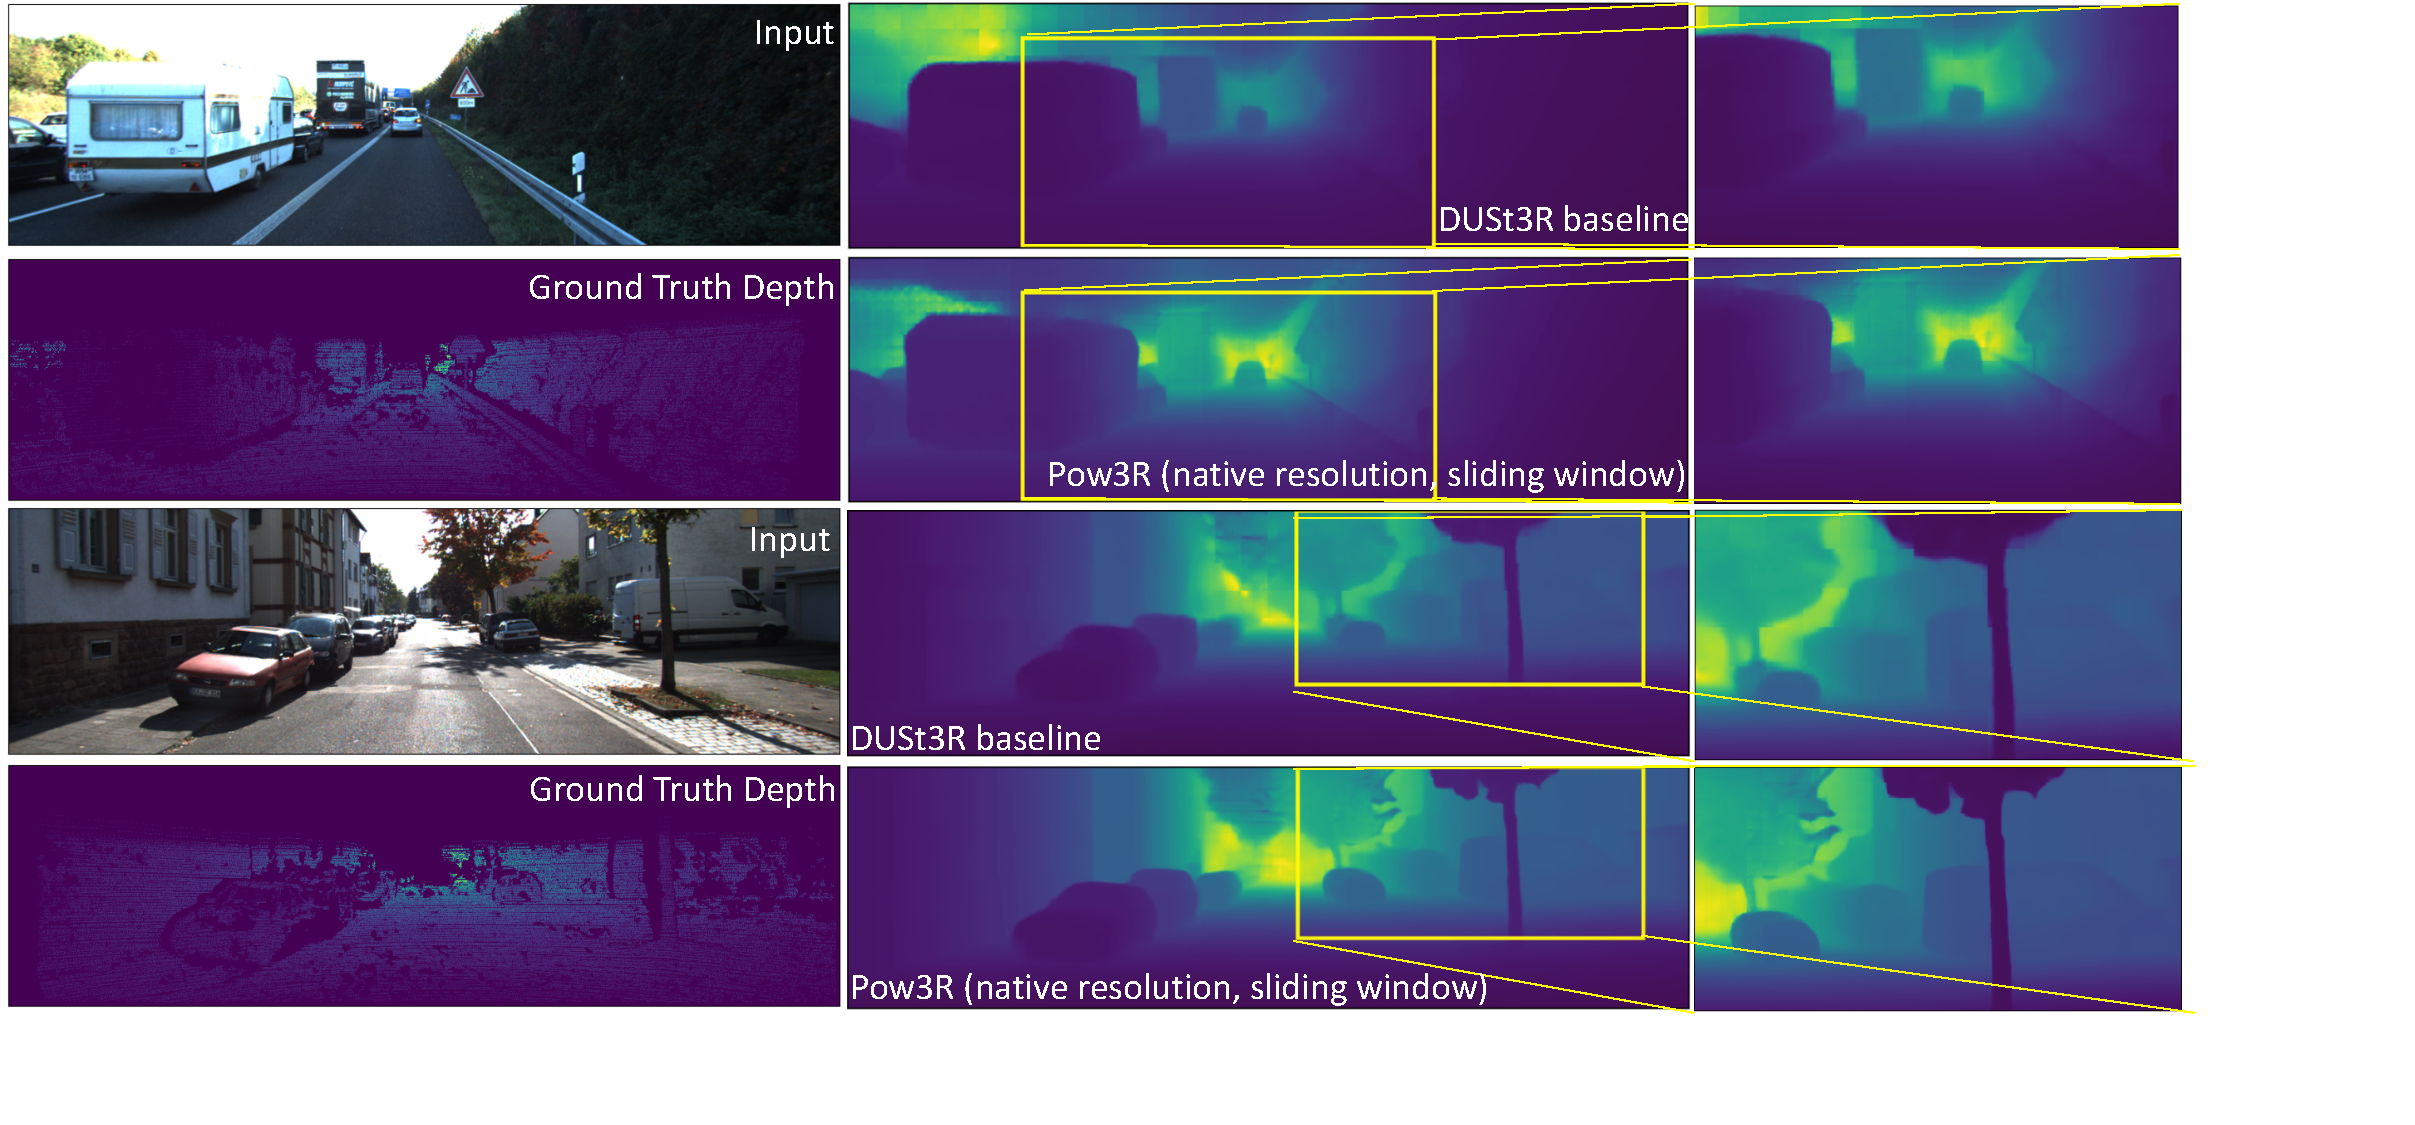
\includegraphics[width=\linewidth,trim=0 50 100 0,clip]{figures/old_supp/kitti.pdf} \vspace{-0.4cm}
    \caption{\textbf{High-resolution with \ours{}: } We adopt the asymmetric sliding approach as in the Figure 4 of the main paper to increase the resolution of pointmaps of a single image. \emph{Please refer to the attached video for more detailed information.}} \vspace{-0.4cm}
    \label{fig:kitti_result}
\end{figure*}

\myparagraph{Reimplementation of Evaluation Code.}
\textit{\duster{}}$^\dagger$ in Table~\ref{tab:mvd_supp} refers to the results reported in the original \duster{} paper, while `\duster{} (repr.)' denotes our re-implementation.
After observing that our re-implementation with the official code and checkpoint reaches better performance than the ones published, we have communicated with the authors to check for any issue. Authors have confirmed the presence of a bug in their internal codebase that was the cause of performance degradation.


\section{High-resolution processing with \ours{}}

\myparagraph{Overall.} 
Providing camera intrinsics as auxiliary input enables us to upsample the pointmaps by sequentially processing crops in a sliding window scheme. This is feasible since we train on non-centered cropped images along with their camera intrinsics.
As explained in Section 3.1 of the main paper, we densify the camera intrinsics as rays, and feed them in the encoder.
This allows us to deal with arbitrary aspect ratios and high-resolution images by processing image crops, which \duster{} is not capable of. A full resolution processing is not possible neither at test time nor at train time. This is clearly shown in Table 2 of the main paper, where naively feeding the high-resolution images to a low-resolution network degrades performance. Likewise, training on high resolution images is computationally prohibitive. Our multi-stage schemes, based on smaller crops, allow for processing full resolution images, without training in such high resolutions. 

\myparagraph{Asymmetric sliding.}
There are various ways to perform high-resolution processing.
In the monocular case where we would like to upsample pointmaps, we feed a downsampled coarse input image alongside the same high-resolution cropped image as shown in Figure 4 of the main paper or in \cref{fig:kitti_result} of this Supplementary.

\myparagraph{Coarse-to-fine strategy.}
Alternatively, we can feed two high-resolution image crops to the network, in which case we can condition the outcome based on an initial coarse pass.
Here, conditioning consists in feeding coarse depthmap (estimated during the initial coarse pass, where we simply downscale images) as auxiliary information for the two high-resolution crops.
The resulting pointmaps for each crop are scale-invariant; therefore, we solve their scale by simply computing the median scale factor in overlapping areas.
\emph{We refer to the attached video for additional details and visualizations.}



\myparagraph{KITTI.}
The KITTI dataset, with its unique resolution of $370\times1226$, and non-typical aspect ratio, presents a challenging test-case in a zero-shot settings. 
Using our coarse-to-fine approach, we can handle high-resolution images efficiently and produce detailed and accurate outputs as the Figure 4 of the main paper, as well as in Figure \ref{fig:kitti_result}.

\section{Controllability}

In Section 4.1 of the main paper, we quantitatively evaluate the controllability of \ours{} in Figure 6 of the paper.
In other words, we study what happens when the provided auxiliary information deviates too much from its true ground-truth value.

\myparagraph{Video results.}
\emph{We refer to the attached video showcasing the impact of providing auxiliary information for a given image pair from MegaDepth (validation set) in terms of global 3D reconstruction error.}
We observe that providing intrinsics and pose leads to noticeable improvements yet the largest impact is clearly attained when providing sparse depth, especially for pairs with large depths of field.

\myparagraph{Extreme cases.}
We also show qualitative results in \cref{fig:rot_test,fig:rot_test2}.
The model adheres to the guidance until it reaches a breaking point, at which point it stops functioning normally and output broken pointmaps with very low associated confidence maps, as exemplified in \cref{fig:rot_test2} for $f^1/f^1_{gt}=0.1$.


\begin{figure*}
    \centering
    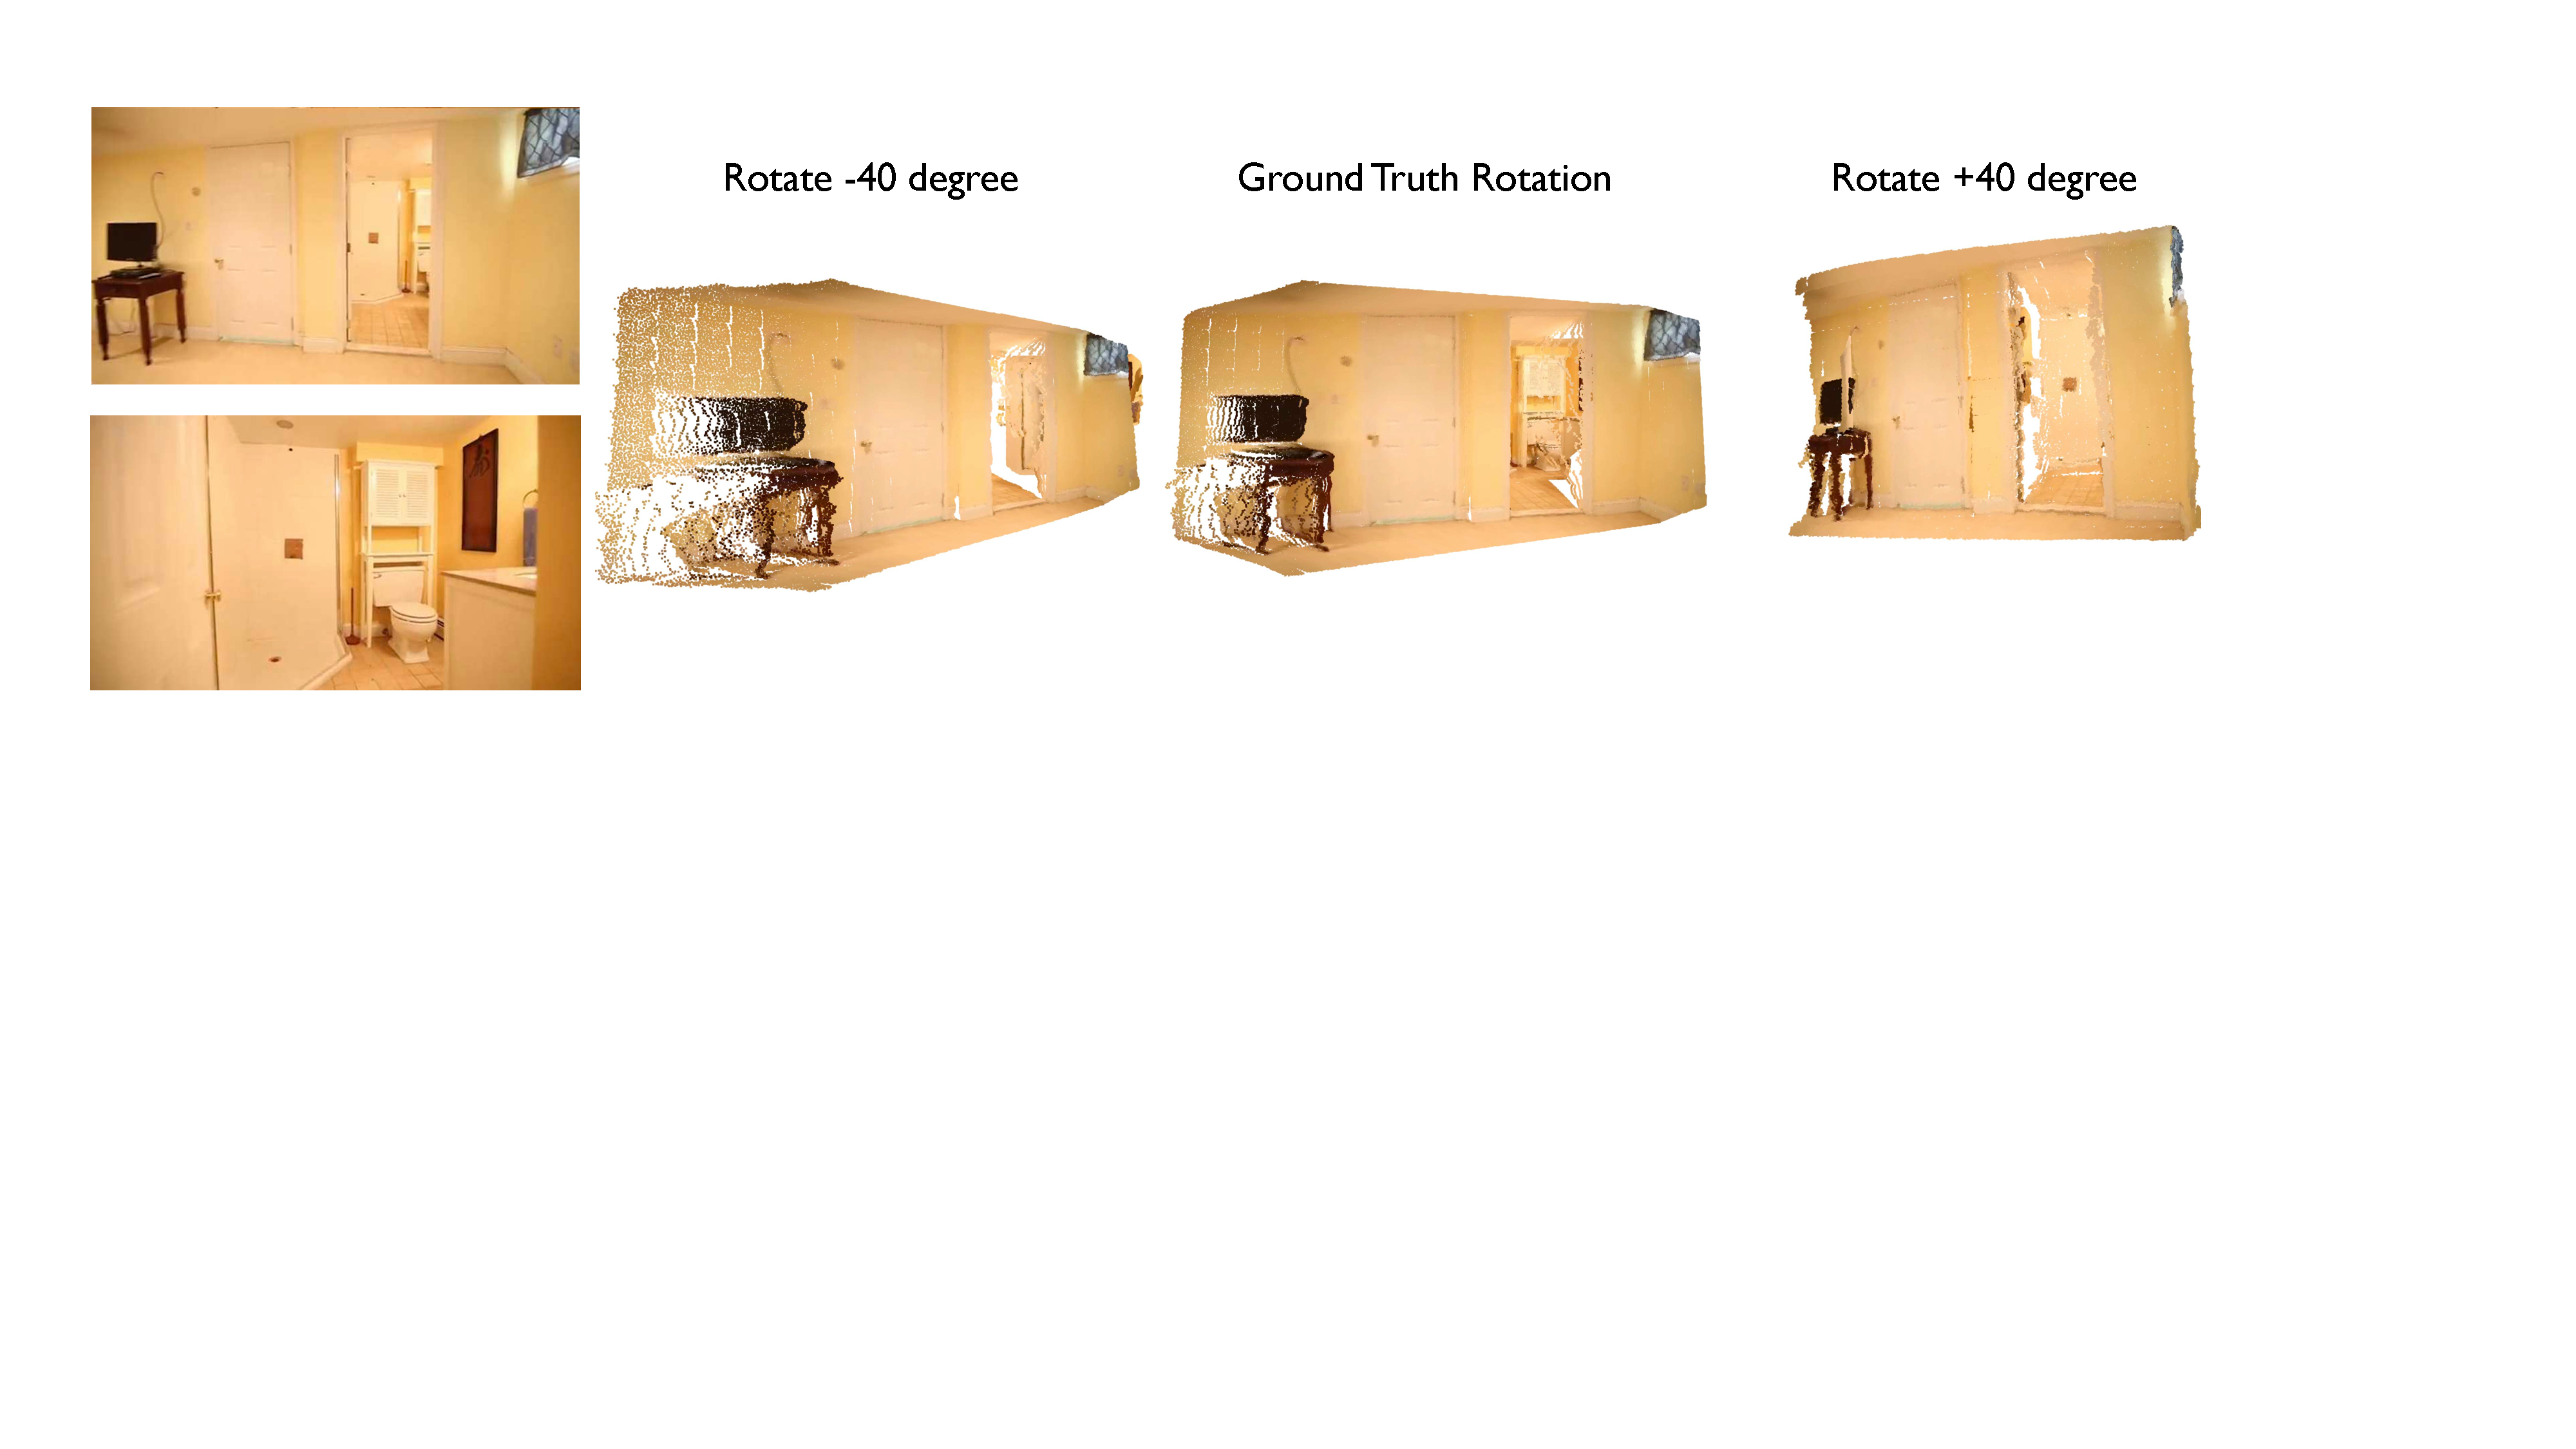
\includegraphics[width=\linewidth,trim=0 500 250 0,clip]{figures/supp/rot_test.pdf} \vspace{-1.2cm}
    \caption{\textbf{Controllability test on rotation: } We provide incorrect camera rotation by -40 degree and 40 degree along y axis each in addition to the ground truth rotation, and render all of scenes from the same location. The quality of reconstruction decreases as the camera rotation deviates from the ground-truth. }
    \label{fig:rot_test}
\end{figure*}
\begin{figure*}
    \centering
    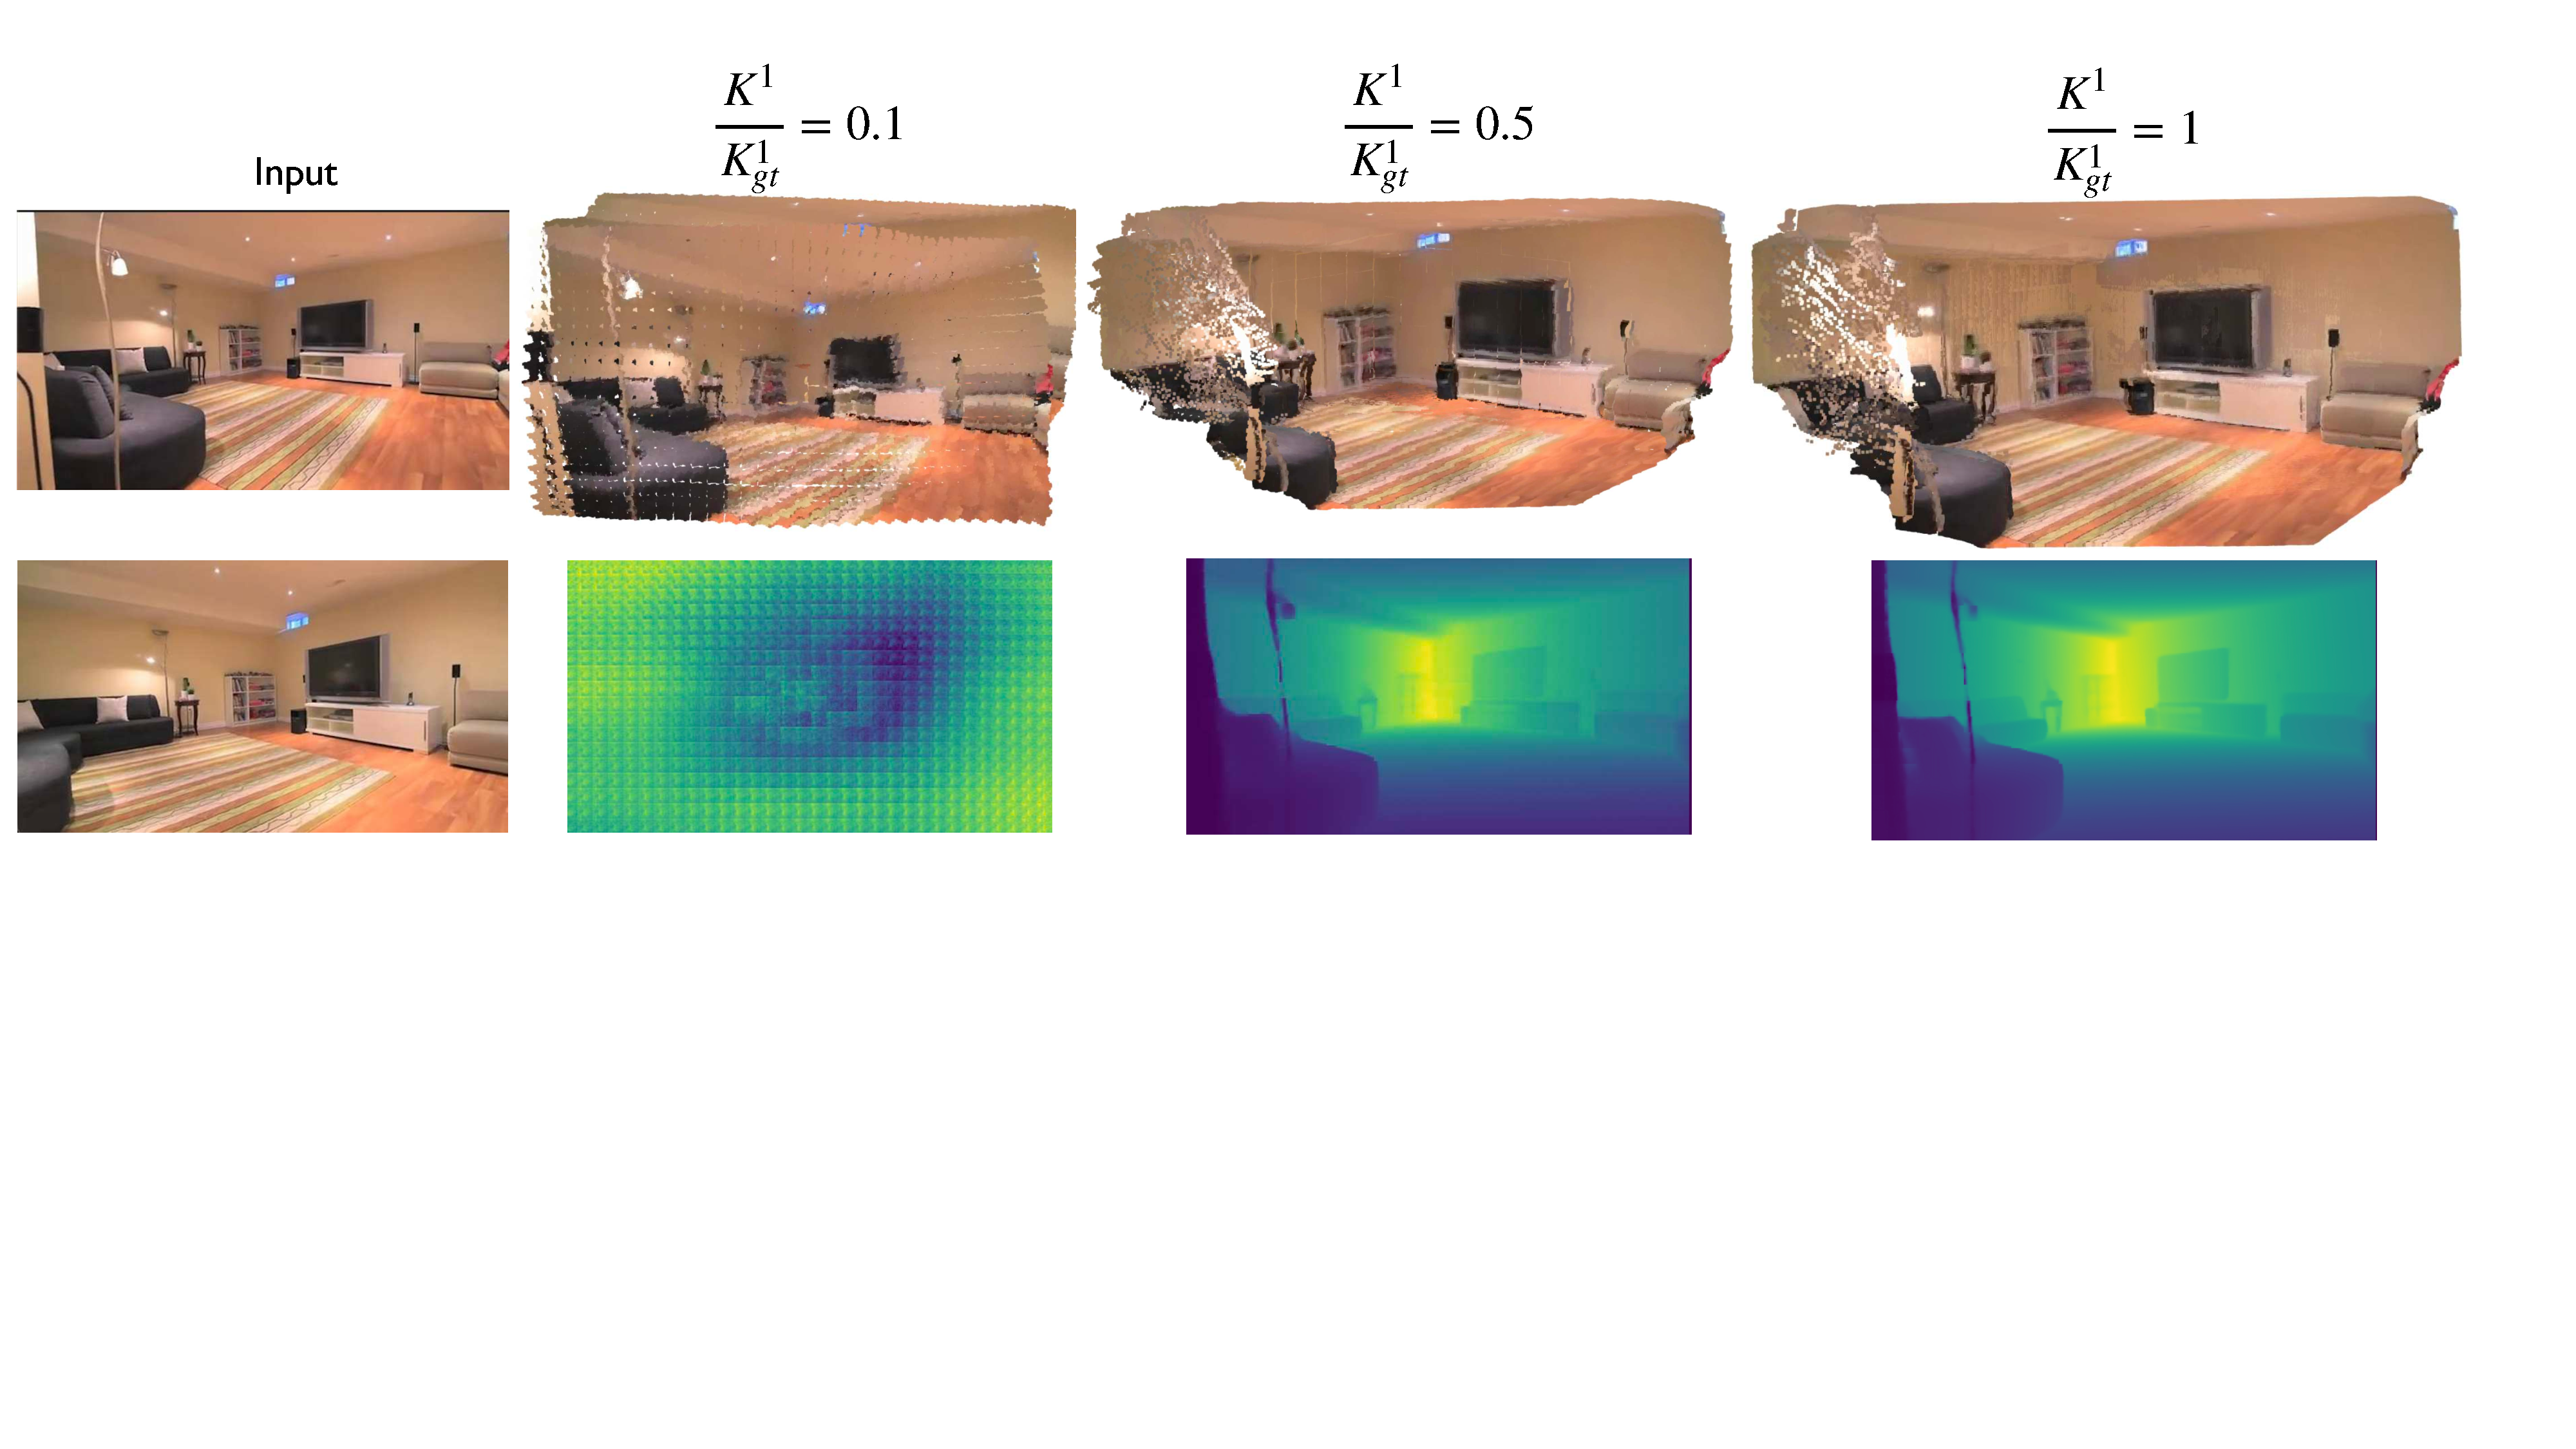
\includegraphics[width=\linewidth,trim=0 500 150 0,clip]{figures/supp/focal_test.pdf}
    \vspace{-0.5cm}
    \caption{\textbf{Controllability test on focal: } We feed incorrect focal length on $K^1$, while providing the second camera with the ground-truth $K^2$. The model fails to generate accurate pointmaps for blatantly false input focals, \eg when the focal $f^1$ is set to $0.1 f^1_{gt}$. 
    The network starts to recover in this case when $f^1 \gtrsim 0.5 f^1_{gt}$.}
    \label{fig:rot_test2}
\end{figure*}


\section{Noises in the ground-truth depth annotation: NYUd - Section 4.1 of the main paper}

\begin{figure*}
    \centering
    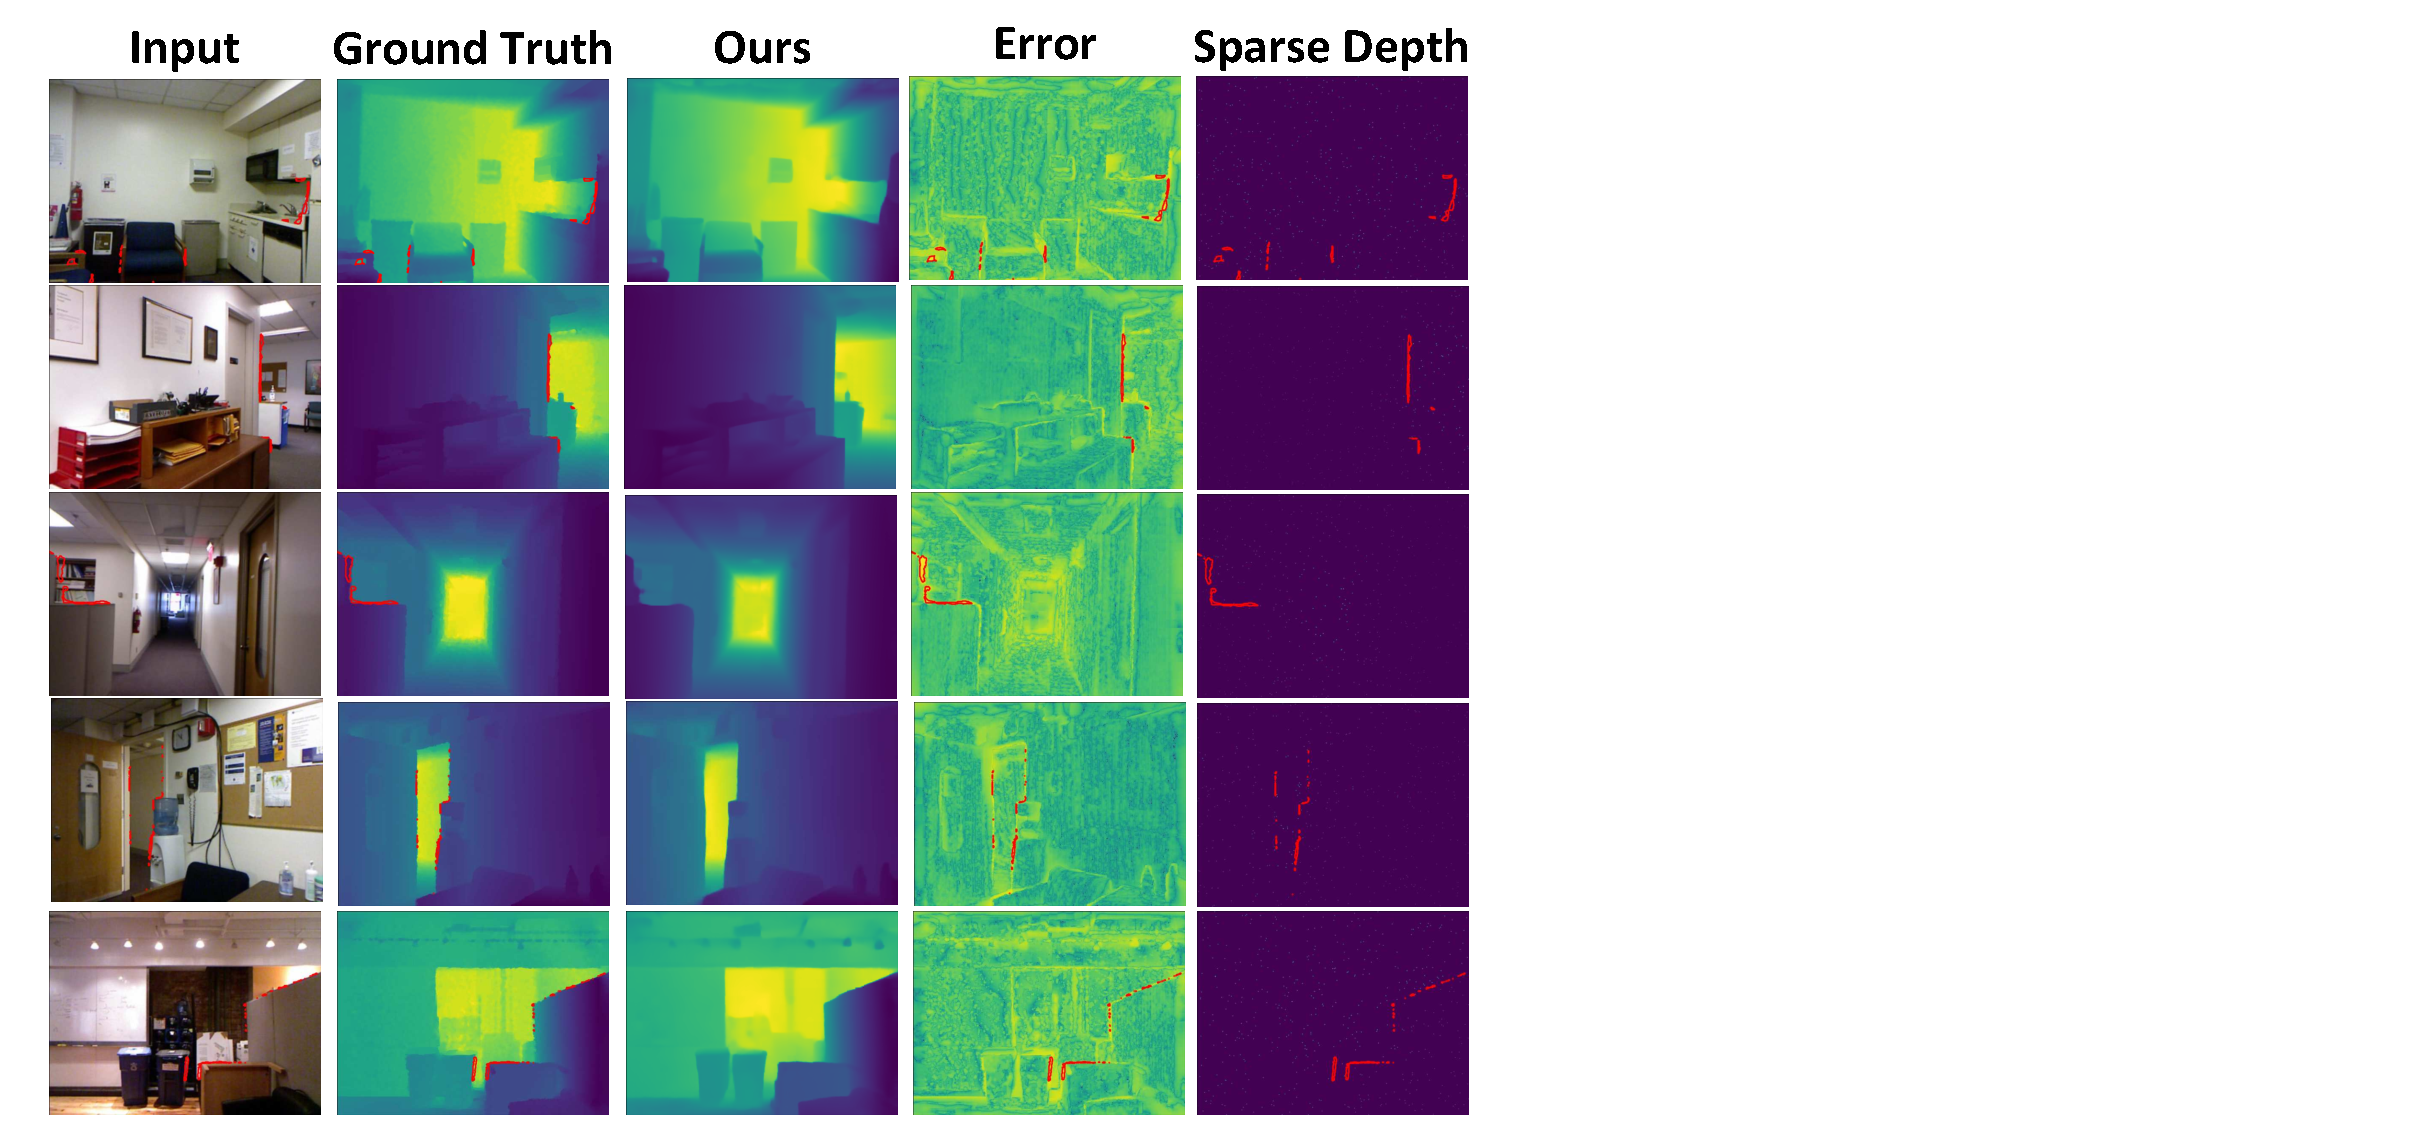
\includegraphics[width=\linewidth,trim=0 0 440 0,clip]{figures/supp/nyud2.pdf}  \\[-0.3cm]
    \caption{
    \textbf{Noise in the Ground-Truth Annotations in NYUd Dataset: } Red contours in input and ground truth show areas where the error is above the threshold. Sparse depth indicates that these inaccurate annotations are not provided as the input to the network. Errors are in log scale, and \ours{} is tested on zero-shot setting.
    }
    \label{fig:nyu_errors}
\end{figure*}

In Figure \ref{fig:nyu_errors}, we highlight the erroneous ground-truth annotations present in the NYUd~\cite{SilbermanHKF12} dataset.
Specifically, the red contours in the visualization indicate regions where the discrepancy between the ground-truth and the predicted depth values exceeds a defined threshold. 
These regions often correspond to areas with edges or fine-structural details, that offer surfaces tangential to the viewing ray, and are not easy to annotate accurately.
As in Figure~\ref{fig:nyu_errors}, \ours{} can inpaint the sparse depthmap consistently and produce high-quality depthmaps. Note again that NYUd dataset is not part of our training set yet
\ours{} performs better than several depth completion models including ~\cite{completionformer2023,guidenet,bpnet,yan2024tri,lrru} across varying input sparsity depth ratios, as illustrated in Figure 5 of the main paper. We posit that a significant portion of the error observed is attributable to the aforementioned  inaccuracies in the ground-truth annotations of NYUd dataset.



\section{Extended Related work}
\label{sec:extended_related}


\myparagraph{Structure-from-Motion.} 
Traditional SfM methods typically involve non-differentiable components, such as keypoint detection, matching, and incremental camera registration; however, VGGSfM~\cite{wang2023vggsfm} integrates recent advancements in deep learning to create an end-to-end trainable system.
Graph attention networks can also be leveraged~\cite{brynte2024learning} to learn SfM by processing 2D keypoints across multiple views, and computing corresponding camera poses and 3D keypoints.
MASt3R-SfM~\cite{duisterhof2024mast3r} integrates SfM pipeline within MASt3R~\cite{leroy2024mast3r}, which eliminates the need for RANSAC by employing robust local reconstructions, and conducts optimization through successive gradient descents, first using a 3D matching loss and then refinining with a 2D reprojection loss.
\ours{} differs from traditional approaches by leveraging attention between image patches along with auxiliary inputs such as camera intrinsics, extrinsics and sparse depths, to discover camera poses directly from pointmaps.

\myparagraph{MVS and 3D reconstruction.} MVS aims to reconstruct dense 3D surface through triangulation from multiple viewpoints, traditionally with hand-crafted features~\cite{furukawa2015multi, galliani2015massively, schonberger2016pixelwise}. 
Learning-based approaches have been incorporated for MVS, followed by the emergence of Neural Radiance Fields (NeRFs) and its extended works~\cite{niemeyer2020differentiable, yariv2020multiview, gu2020cascade, leroy2021volume, peng2022rethinking, yao2018mvsnet, mildenhall2021nerf, sitzmann2019srns}.
The need for camera parameters and sparse scene initialization pushed NeRF and Gaussian Splatting (GS)~\cite{kerbl20233d} based models to leverage SfM pipelines such as COLMAP~\cite{schonberger2016structure}.
The quality of these approaches depends on the accuracy of camera parameters, and the error from cameras is not often rectified during the training.
There have been attempts to update camera parameters while optimizing the 3D scene~\cite{lin2021barf, wang2021nerf, chen2023dbarf, jeong2021self, chng2022gaussian, park2023camp}; however, many of these approaches require known camera intrinsics, good initialization, and usually rely on a weakly supervised photometric loss.
Single-view based approaches~\cite{jang2021codenerf, yu2021pixelnerf,jang2024nvist,lin2023vision,sargent2023vq3d,chen2023explicit, szymanowicz2024splatter, chan2022efficient} have been explored as they are less dependent upon camera poses, but these models usually require aligned datasets or cannot resolve the scene ambiguity completely.
The \duster{} framework departs from these approaches as it aims to do unconstrained 3D reconstruction via supervised pointmap regression, without relying on camera parameters.
In \ours{}, we further develop \duster{} by allowing the network to take auxiliary inputs such as sparse depth, camera intrinsics and camera pose. Naturally incorporating existing scene and camera priors seamlessly with RGB images further improves performance, and importantly it enables full-resolution processing of images, which was not easily achievable prior to this work~\cite{winwin}.

\myparagraph{RGB-to-3D.} 
From a single image, combined with monocular depth estimators and camera intrinsics, networks can predict pixel-aligned 3d point clouds~\cite{bian2022auto, szymanowicz2024flash3d, yin2022towards, yin2021learning}.
SynSin~\cite{wiles2020synsin} does new-view synthesis by predicting depth, generating point clouds, and using the differentiable renderer to synthesize images, and it computes the camera intrinsics by temporal consistency within video frames or off-the-shelf estimator.
For multi-view settings, ~\cite{teed2020deepv2d, ummenhofer2017demon, zhou2018deeptam} have been proposed to build a differentiable SfM, but the camera intrinsics are required.


\myparagraph{Focal Estimation.}
Classical approaches rely on parallel lines~\cite{grompone2010lsd} that intersect at vanishing points for single-image calibration, and vanishing point estimations were in~\cite{bernard1983interpreting, kluger2020consac, zhai2016detecting, tong2022transformer}.
Learning-based methods~\cite{lopez2019deep, hold-geoffroy2022deep,zhai2016detecting} were introduced to regress or classify camera parameters into bins, but there were not as accurate as traditional approaches.
Recent methods combine both traditional and learning-based approaches~\cite{zhu2023tame, veicht2024geocalib}. In our case, the focal length can be directly recovered from the pointmap representation; Our contribution is orthogonal to these lines of work in the sense that \ours{} optionally incorporate sparse depth and relative pose to improve the quality of prediction, again unlike~\duster{}.



\myparagraph{Guiding 3D.} 
Several Simultaneous Localization and Mapping (SLAM) methods incorporate both RGB and RGB-D images like ORB-SLAM2~\cite{mur2017orb}.
DROID-SLAM~\cite{teed2021droid} is a neural-network based system for SLAM that process visual data from monocular, stereo and RGB-D cameras, and it can leverage stereo or RGB-D inputs at test time indifferently. These pipelines however are heavily engineered. In this work, we wish to follow the philosophy from \duster{} where a single network regresses all relevant information, optionally leveraging auxiliary information. %



















\begin{figure*}
    \centering
    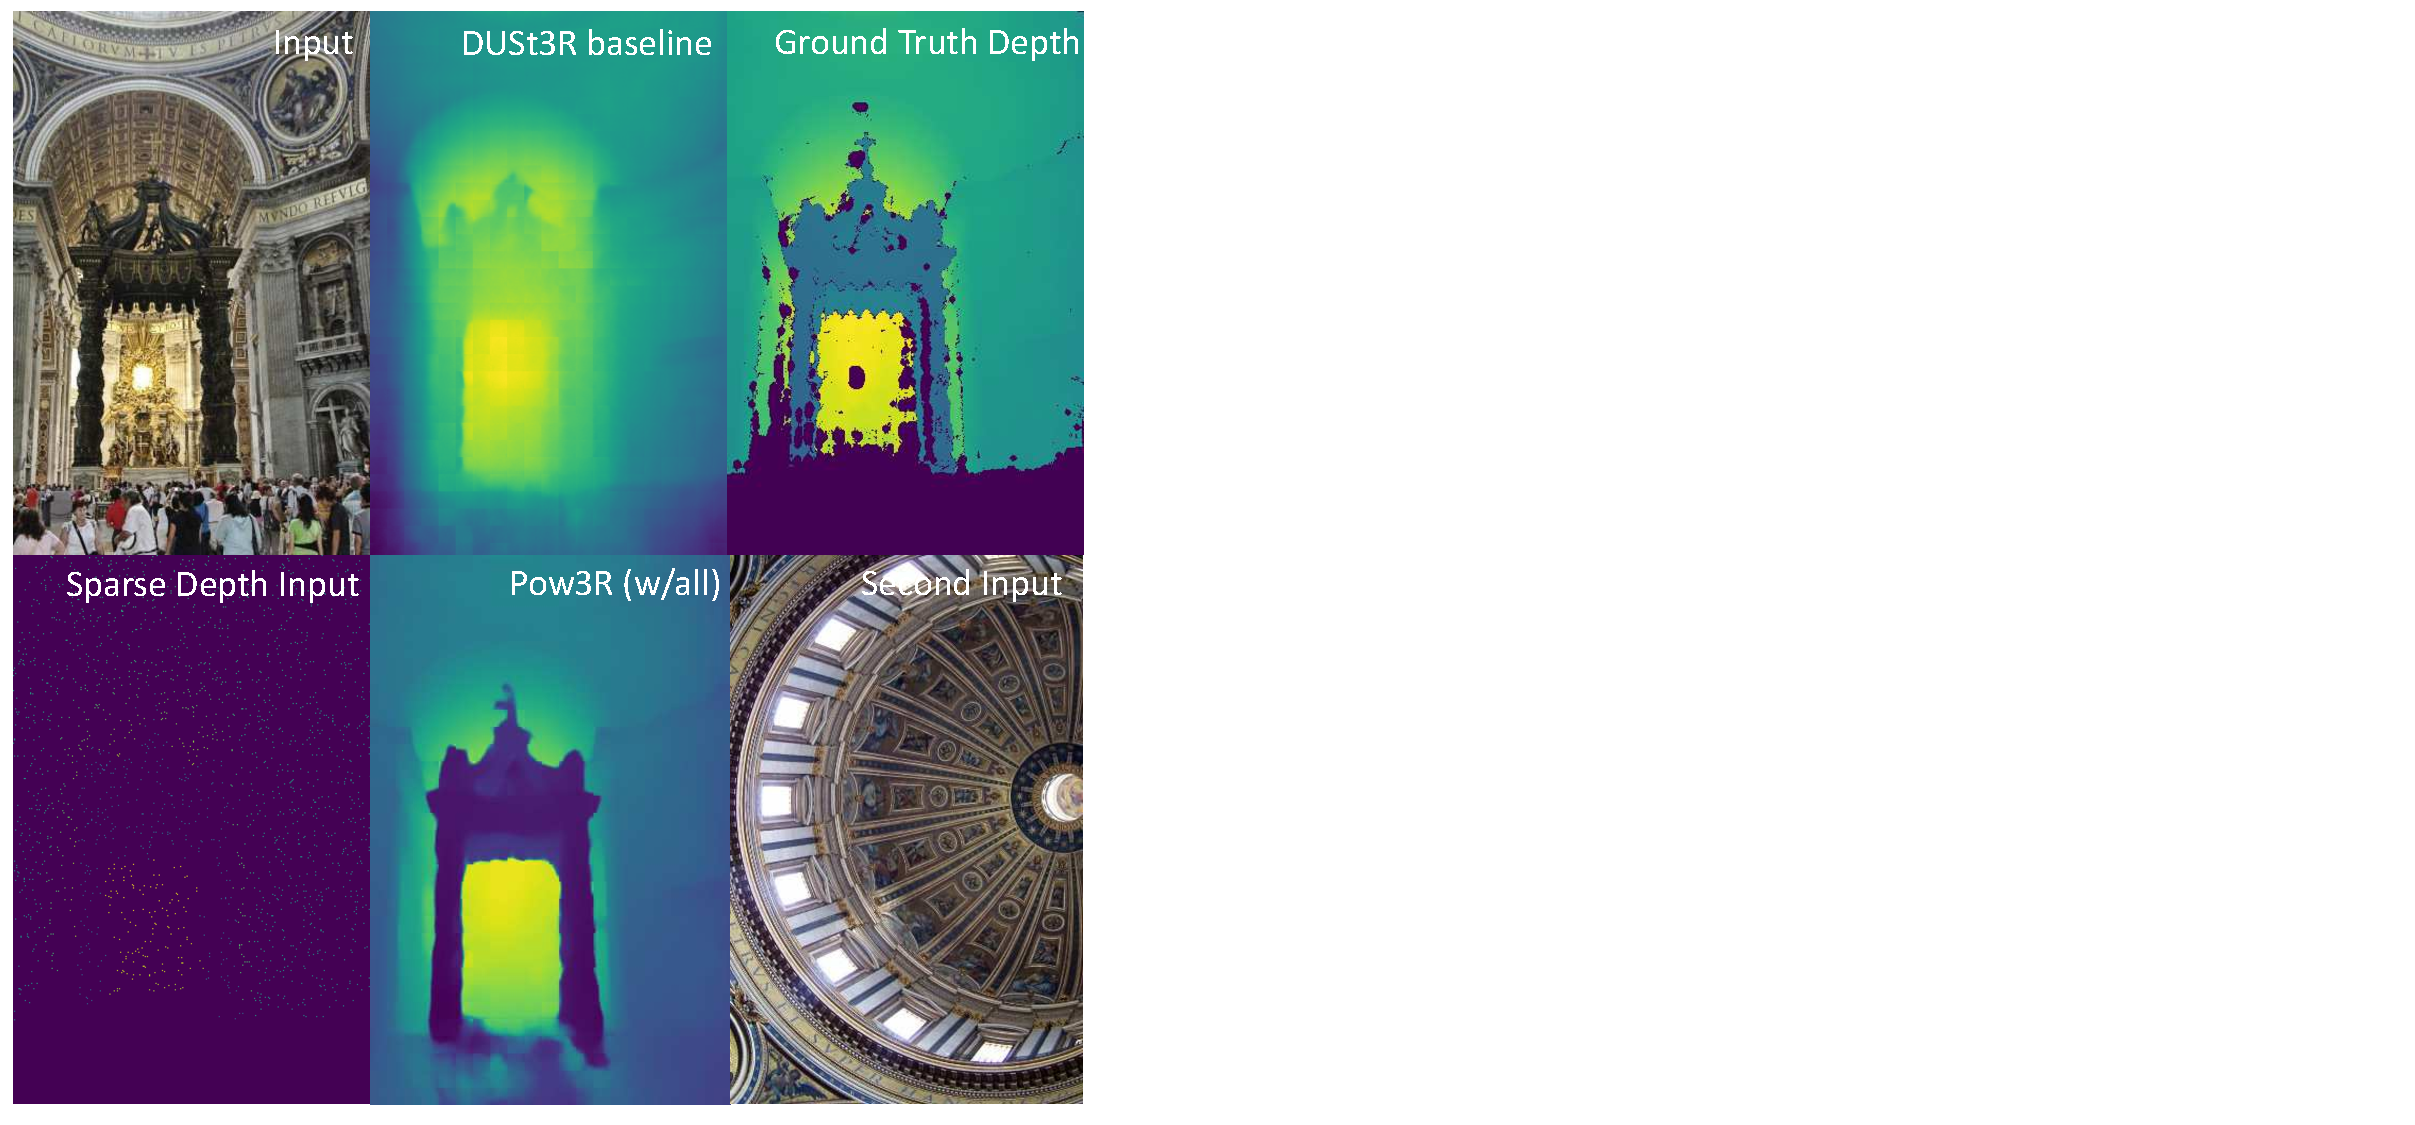
\includegraphics[width=0.7\linewidth,trim=0 0 630 0,clip]{figures/supp/megadepth-gate.pdf} \vspace{-0.5cm}
    \caption{\textbf{Qualitative Result on depthmap.} We validate \ours{} with \duster{} on a Megadepth~\cite{li2018megadepth} indoor scene. Here, we provide camera intrinsics, pose and 2048 sparse point clouds. The result shows that \ours{} can reconstruct the gate properly and smoother than the ground point clouds. In contrast, \duster{} struggles to generate the gate properly.}
    \label{fig:qualitative_megadepth_gate}
\end{figure*}

\section{More Qualitative Results}

We showcase the impact of \ours{} when combined with auxiliary input. 
In the following, we provide examples results both in terms of depthmap and pointmap predictions. 
For each figure, the auxiliary information given to the network are the intrinsics, relative poses and $2048$ sparse depth values except RealEstate10K~\cite{realestate10K} for which no depth information is available.

\myparagraph{Using sparse depthmaps.}
We compare depthmaps predicted by from \ours{} and \duster{} in terms of visual quality in Figures~\ref{fig:qualitative_megadepth_statue},~\ref{fig:qualitative_megadepth_gate},~\ref{fig:qualitative_blendedmvs_statue},~\ref{fig:qualitative_arkit_room}.
Results for \ours{} are consistently better, with much less failure cases than with \duster{}, which is expected given \ours{} receives additional priors.




\begin{figure*}
    \centering
    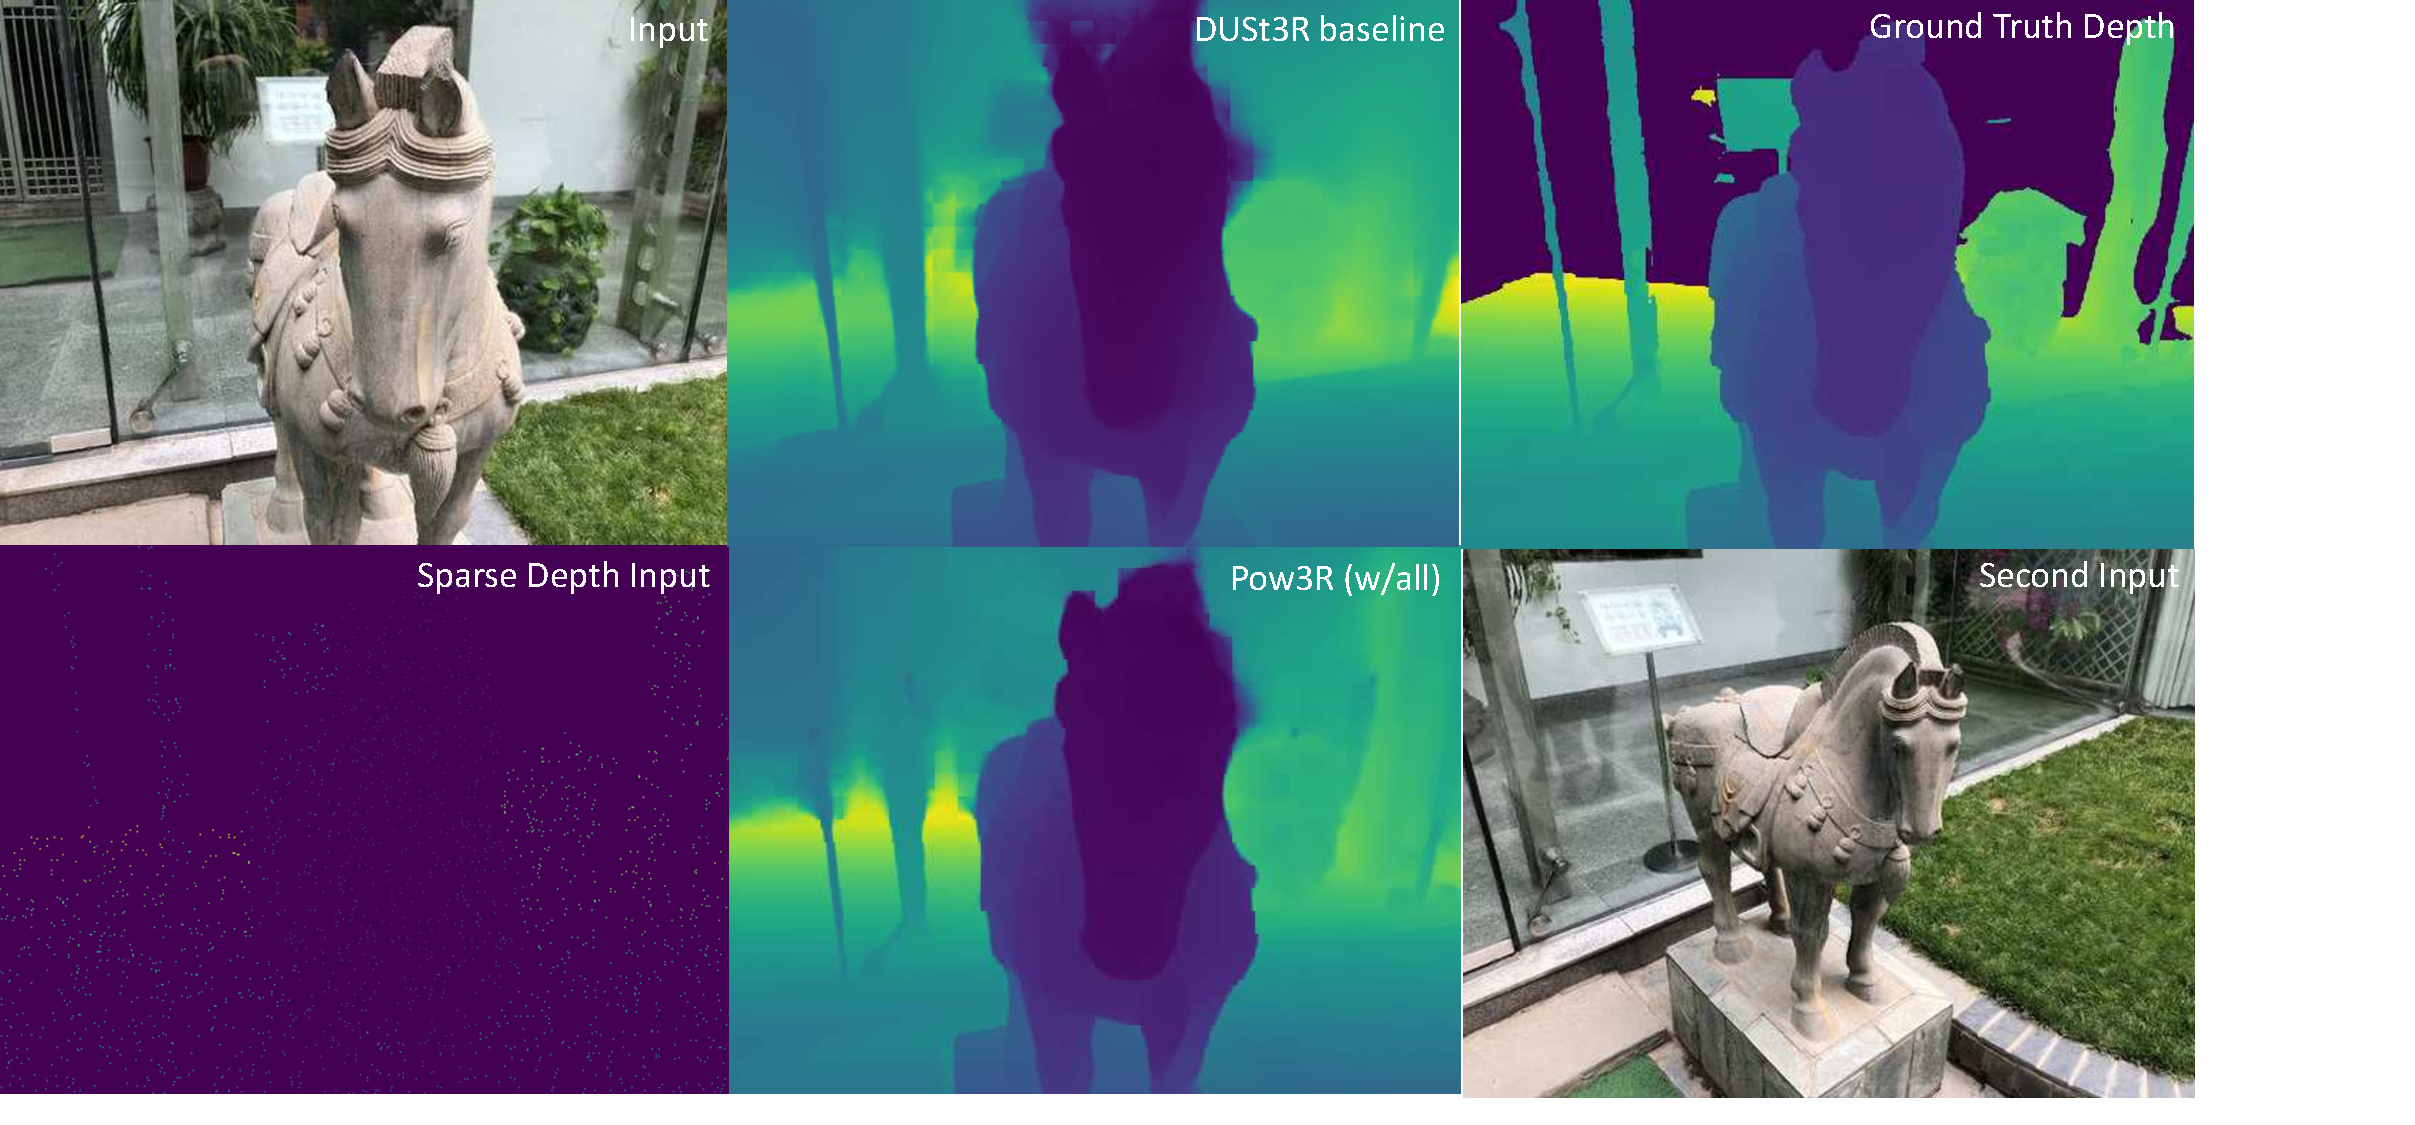
\includegraphics[width=\linewidth,trim=0 0 110 0,clip]{figures/supp/blendedmvs.pdf} \vspace{-0.8cm}
    \caption{\textbf{Qualitative Result on depthmap.} We compare \ours{} with \duster{} on one of the BlendedMVS~\cite{yao2020blendedmvs} scenes. For \ours{}, we provide camera intrinsics, extrinsic and 2048 sparse point clouds. While \duster{} is able to capture the overall scene, it fails to correctly reconstruct the head  of the horse. In contrast, \ours{} delivers a more precise reconstruction. }
    \label{fig:qualitative_blendedmvs_statue}
\end{figure*}

\begin{figure*}
    \centering
    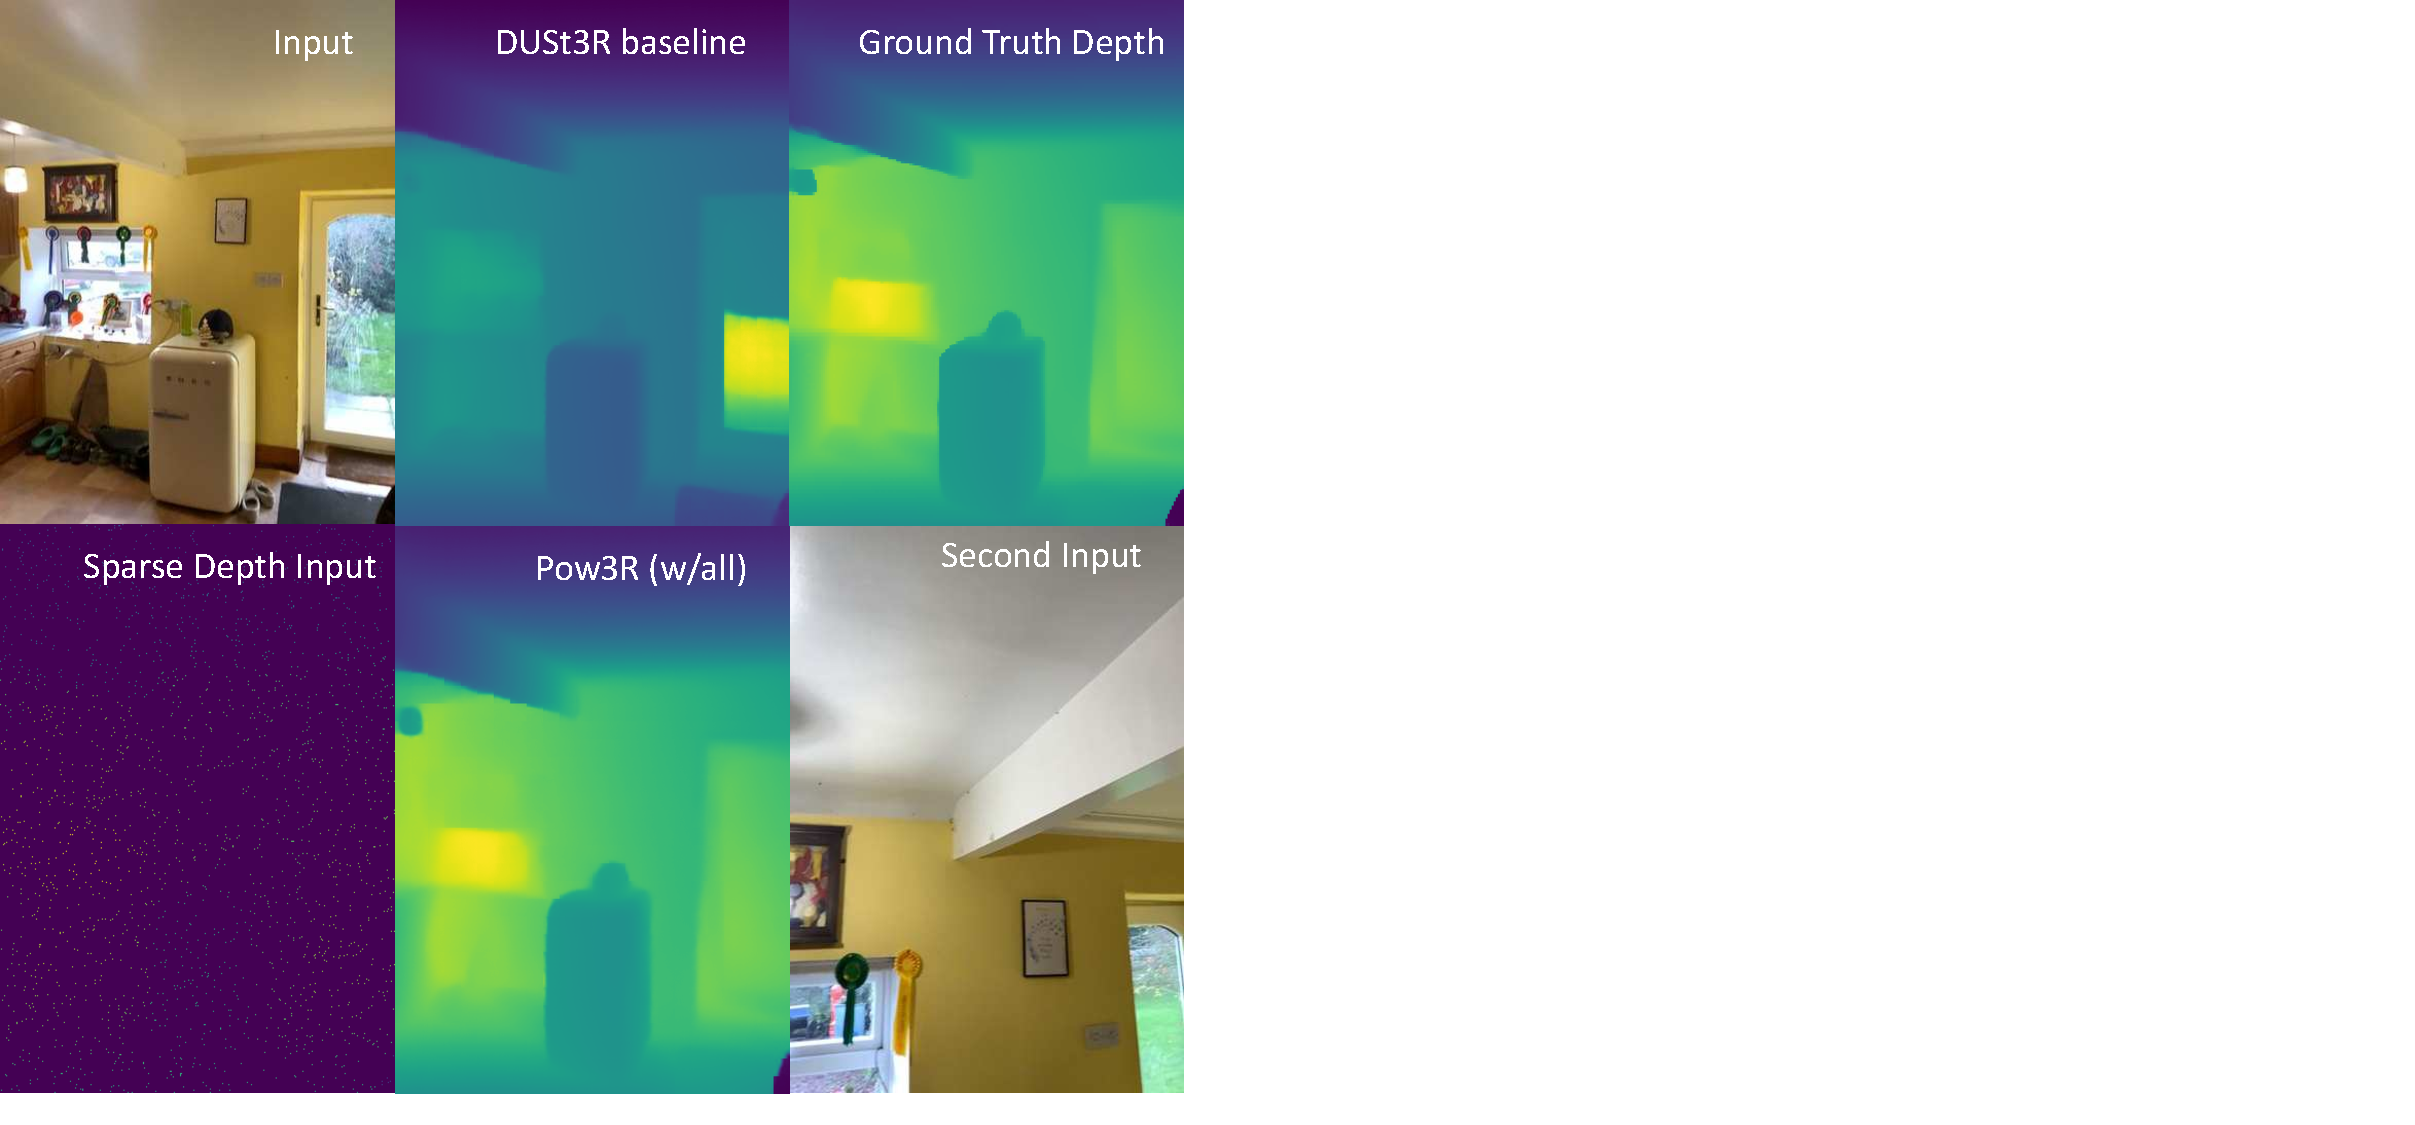
\includegraphics[width=0.8\linewidth,trim=0 0 580 0,clip]{figures/supp/arkit.pdf} \vspace{-0.5cm}
    \caption{\textbf{Qualitative Result on depthmap.} We evaluate \ours{} against \duster{} on an indoor scene from the ARKit~\cite{baruch2021arkitscenes} dataset.%
    We feed to \ours{} camera intrinsics, pose and 2048 sparse depthmap. While \duster{} generally builds a good depthmap, but \ours{} faithfully reconstructs the glass window of the door and small objects on the fridge.}
    \label{fig:qualitative_arkit_room}
\end{figure*}

\begin{figure*}
    \centering
    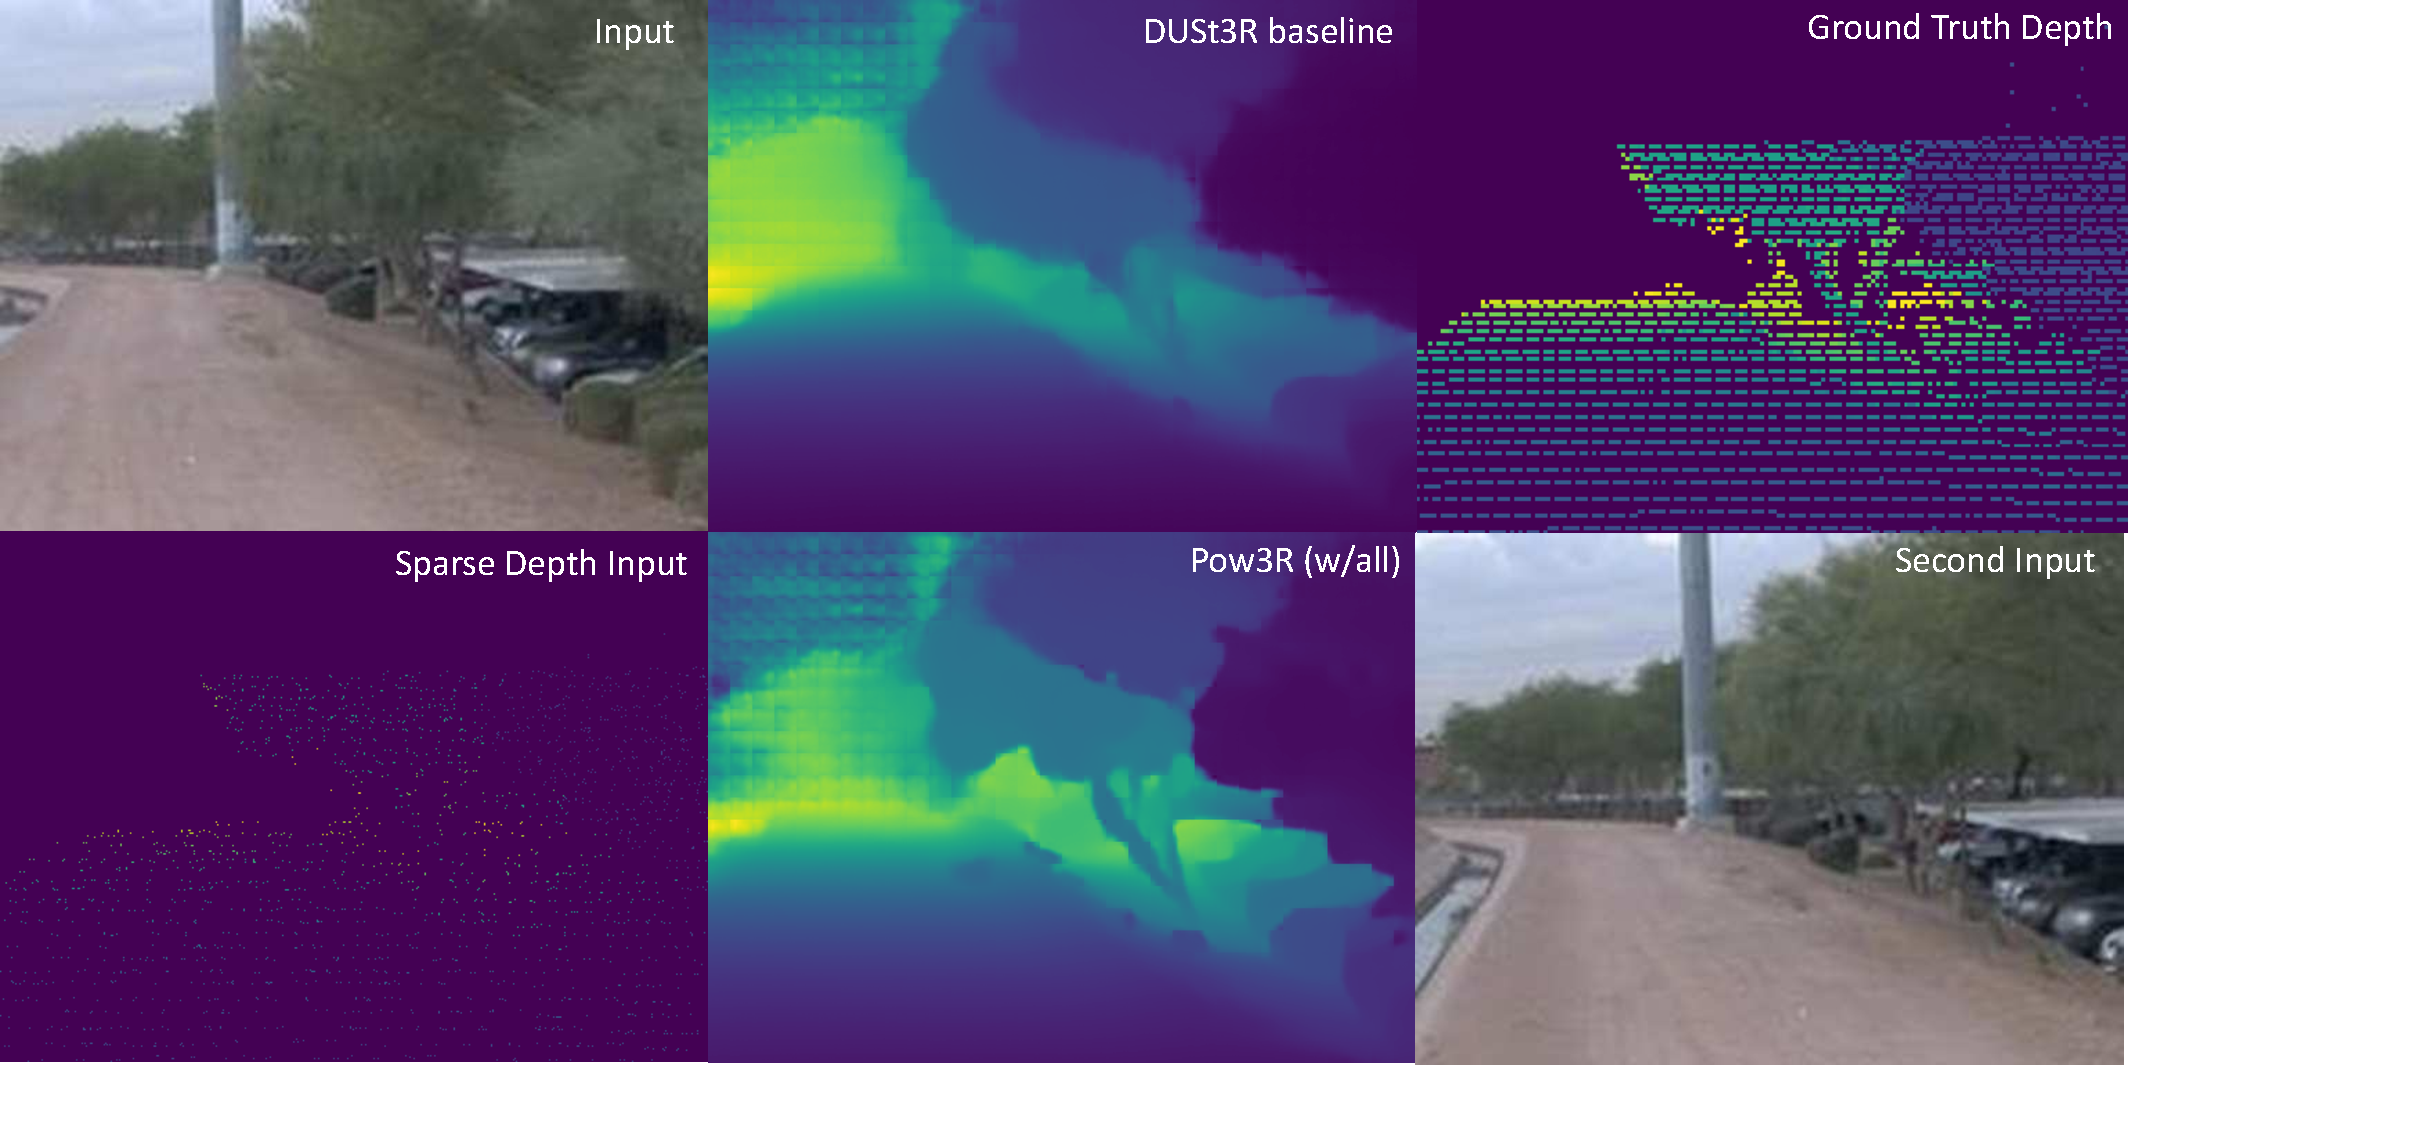
\includegraphics[width=\linewidth,trim=0 50 130 0,clip]{figures/supp/waymo.pdf} \vspace{-0.5cm}
    \caption{\textbf{Qualitative Result on depthmap.} We conduct a comparison on an outdoor scene from the Waymo~\cite{sun2020scalability} dataset. We provide to \ours{} the camera intrinsics, pose and 2048 sparse point clouds from LiDAR. While \duster{} generates a good depthmap from RGB images only, \ours{} shows better performance at capturing details of cars in the parking lot and trees.}
    \label{fig:qualitative_waymo_outside}
\end{figure*}



\myparagraph{Visualizing 3D pointmaps with Cameras.}
Likewise, we showcase the impact of auxiliary information against \duster{}, this time in terms of overall 3D reconstruction as well as camera locations in Figures~\ref{fig:qualitative_megadepth},\ref{fig:qualitative_blendedmvs},\ref{fig:qualitative_megadepth2},\ref{fig:qualitative_re10k},\ref{fig:qualitative_arkit}.
\ours{} reconstructs 3D scenes better than \duster{} in general, while \duster{} generates 3D scenes almost on par with \duster{} in some indoor scenes like Figures~\ref{fig:qualitative_re10k},~\ref{fig:qualitative_arkit}.
Even in these scenes, \ours{} predicts the camera location more precise than \duster{}, which demonstrates that \ours{} performs better with more auxiliary inputs.






\begin{figure*}
    \centering
    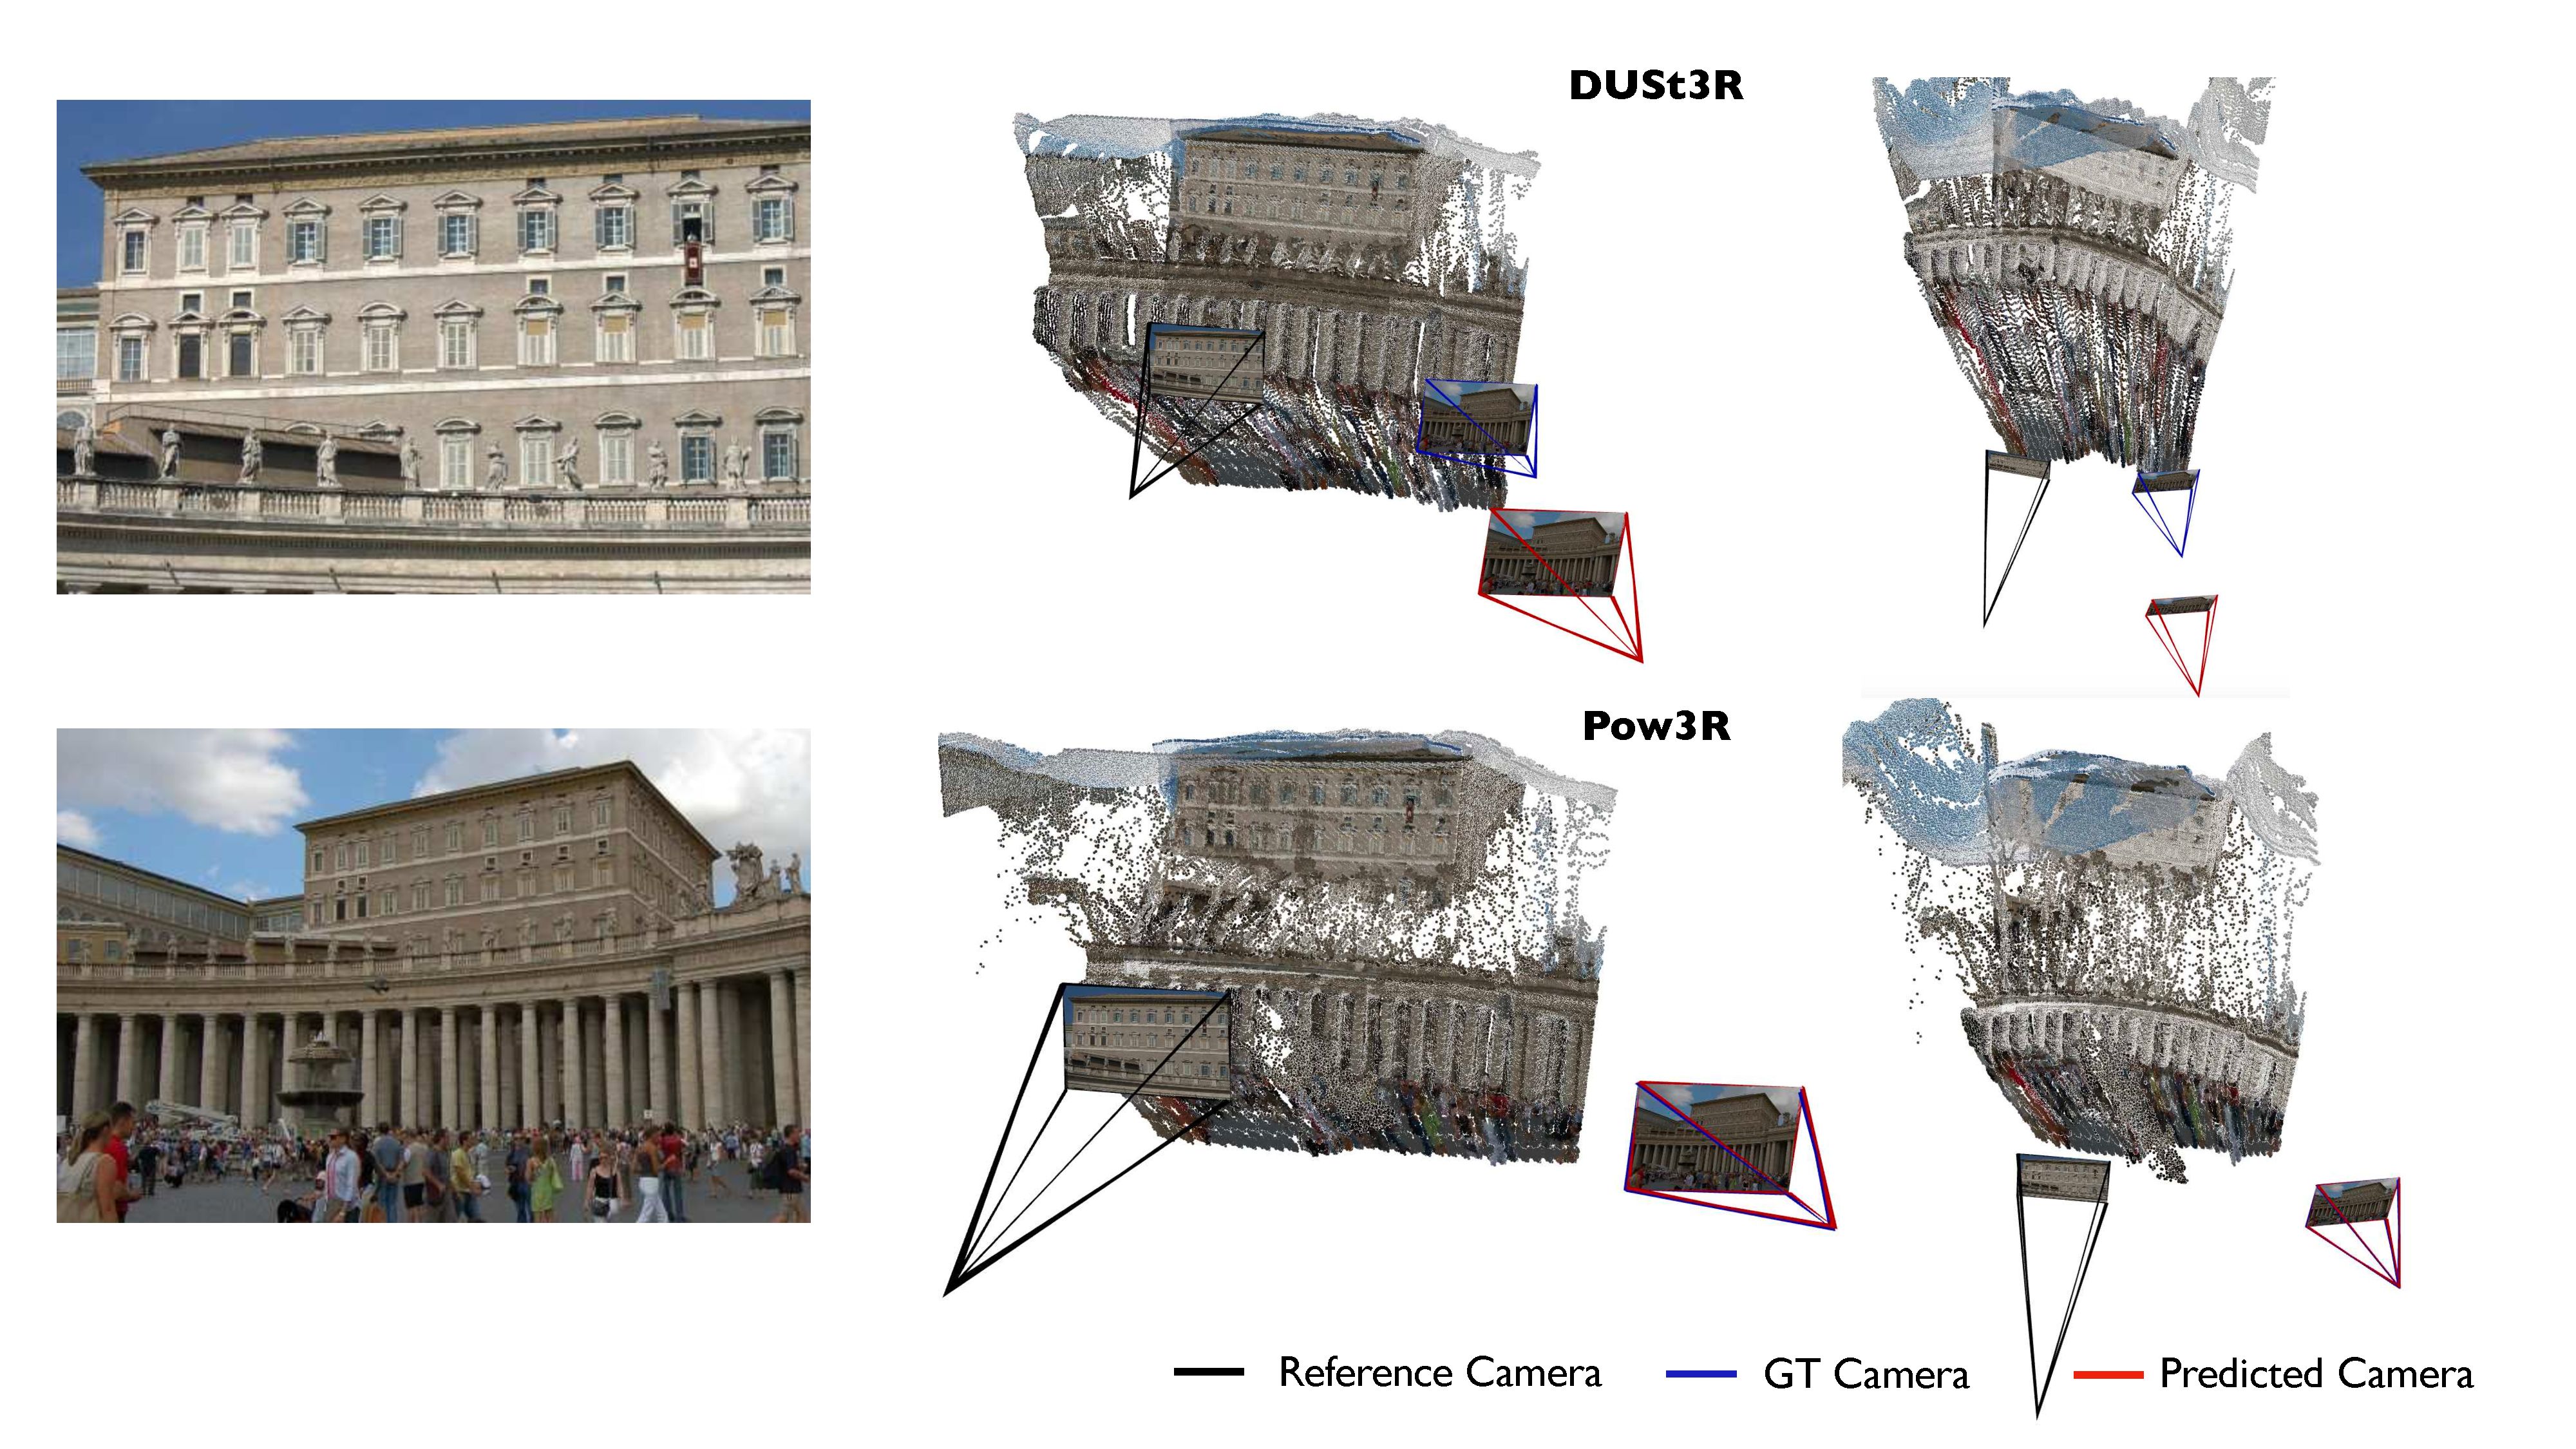
\includegraphics[width=\linewidth]{figures/supp/megadepth_figure.pdf}  \vspace{-0.5cm}
    \caption{\textbf{Qualitative Result on 3D reconstruction and camera estimations.} We evaluate our model on one of the Megadepth~\cite{li2018megadepth} outdoor scenes. Inputs include camera pose, intrinsics as well as 2048 sparse point clouds. While \duster{} attempts to reconstruct the scene from two extreme viewpoints, it struggles with scale ambiguity and improper camera registration. In contrast, \ours{} achieves better reconstruction as well as accurate camera registration.}
    \label{fig:qualitative_megadepth}
\end{figure*}

\begin{figure*}
    \centering
    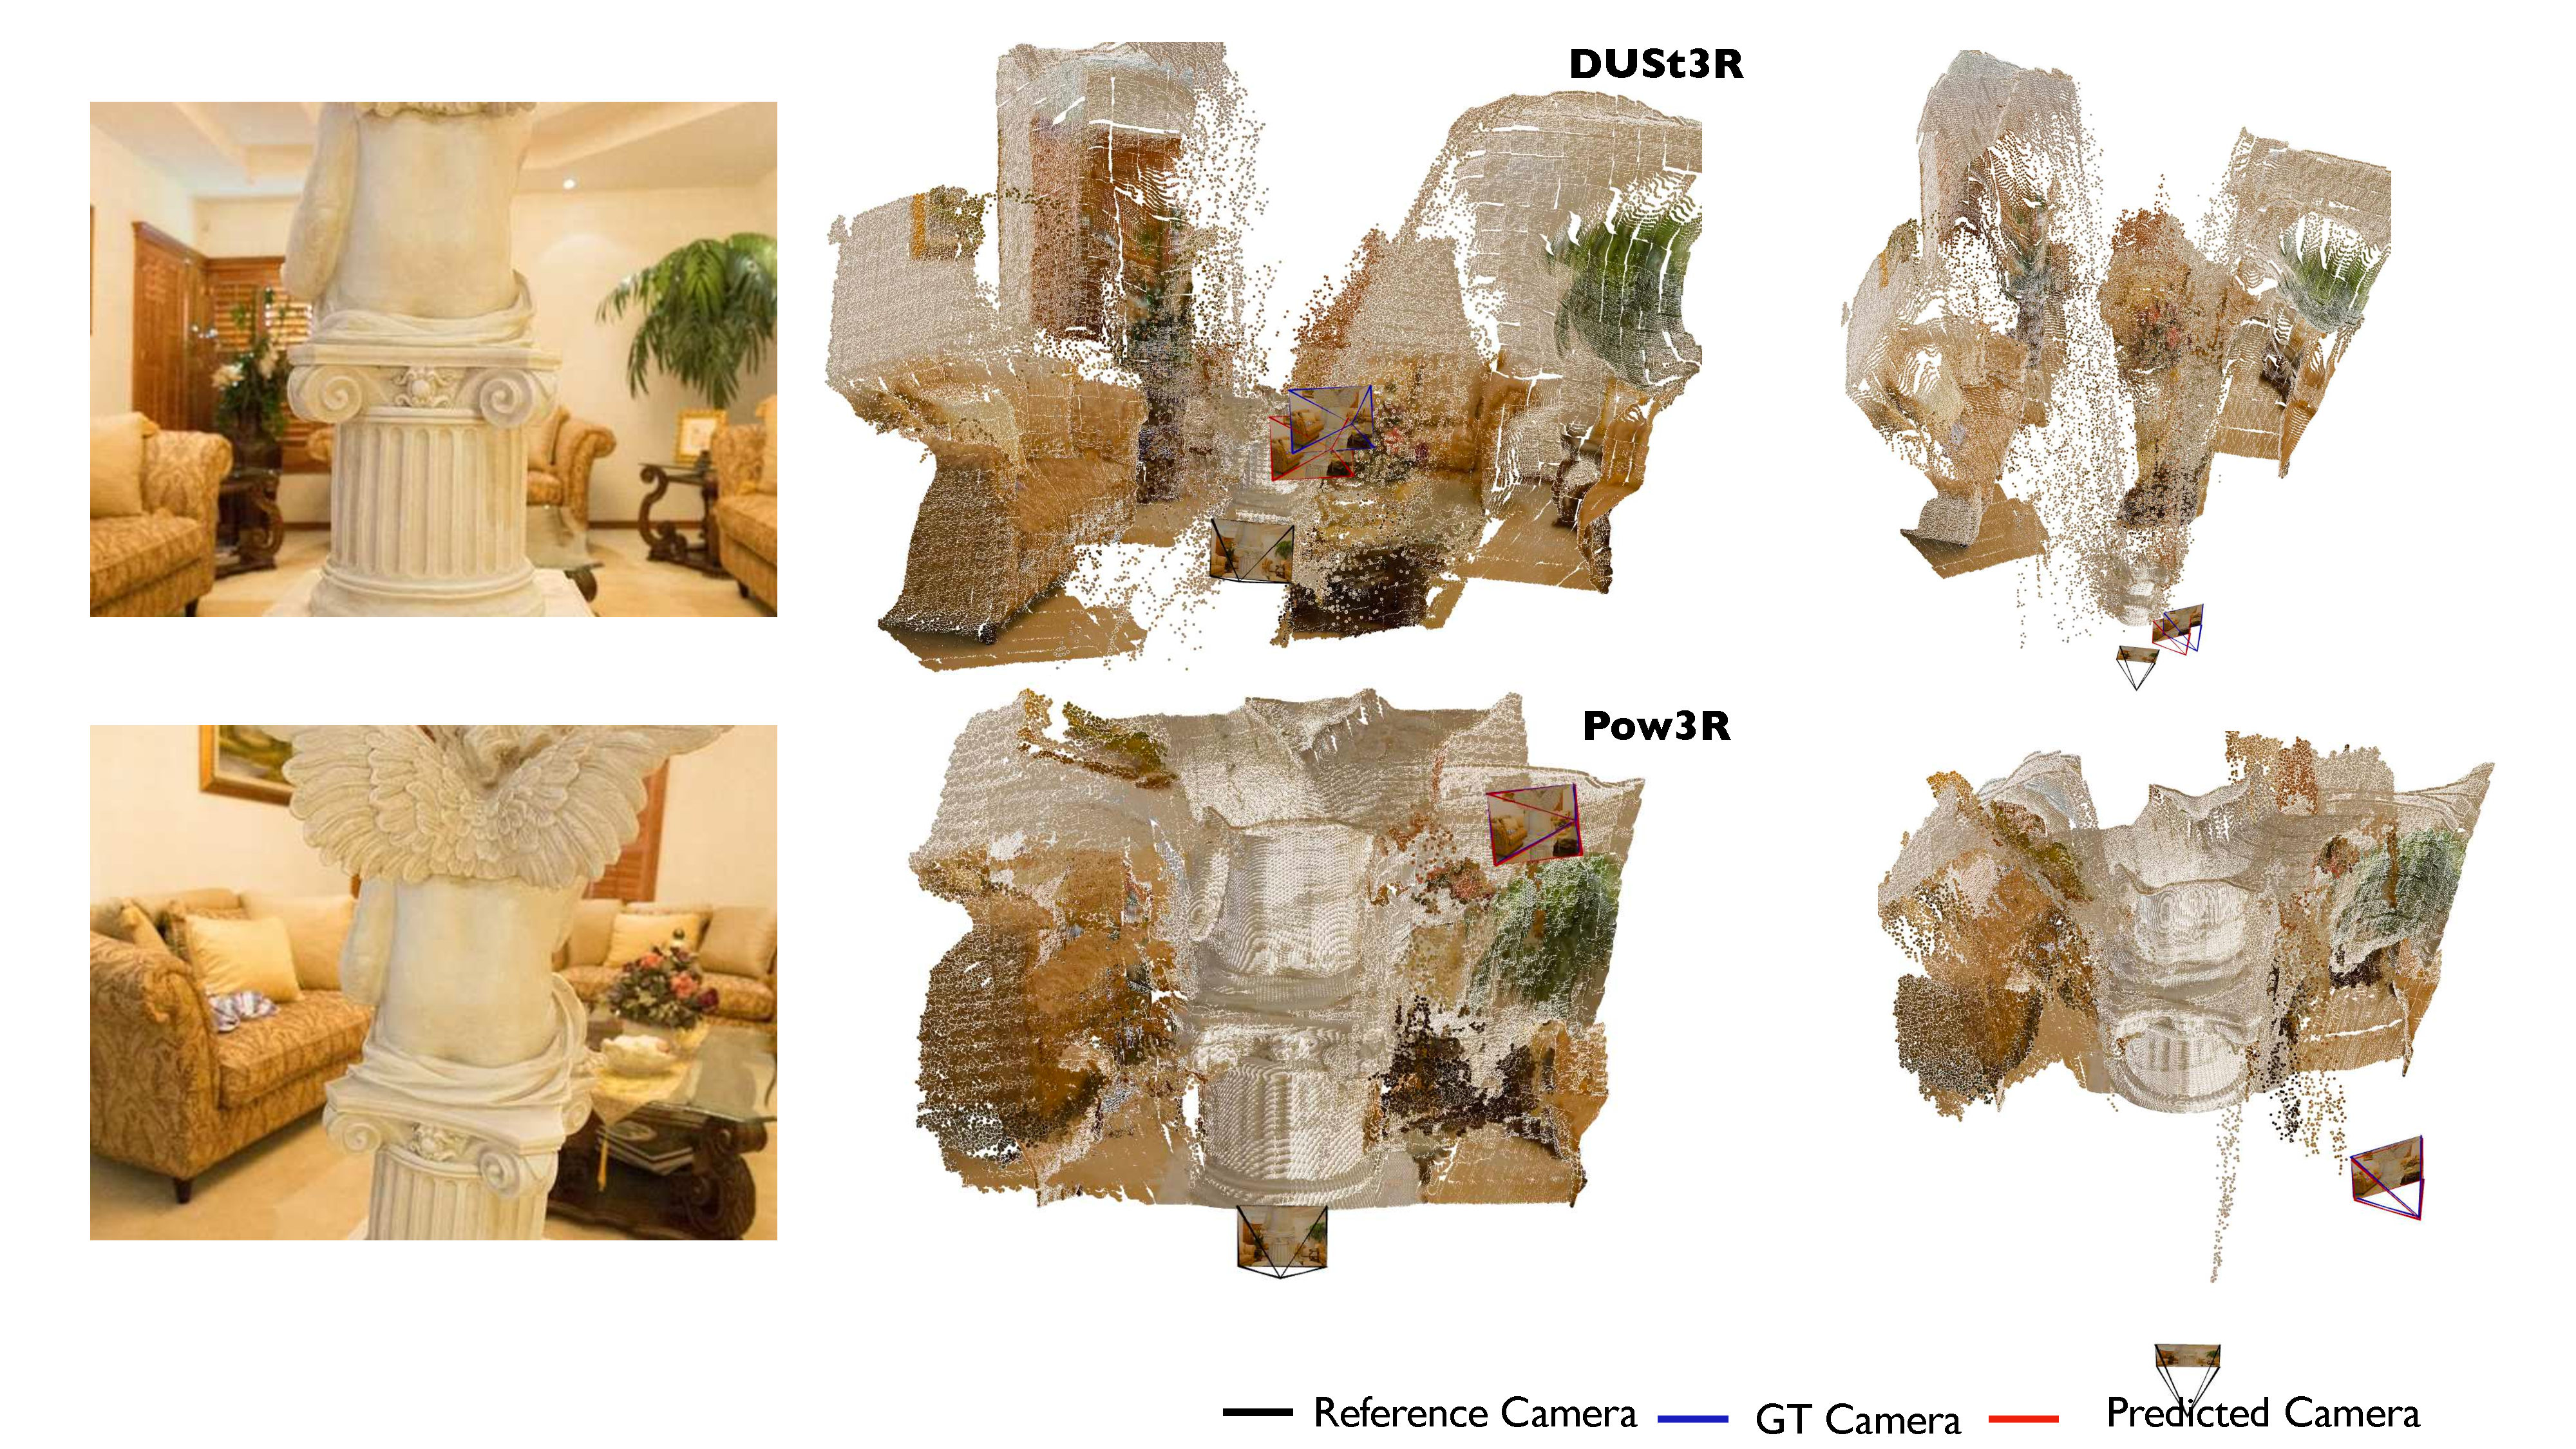
\includegraphics[width=\linewidth]{figures/supp/blendedmvs_figure.pdf} \vspace{-0.5cm}
    \caption{\textbf{Qualitative Result on 3D reconstruction and camera estimations.} We evaluate our model on one of theBlendedMVS~\cite{yao2020blendedmvs} indoor scene. We provide camera intrinsics, extrinsic and 2048 sparse depthmap. While \duster{} incorrectly predicts the depth of field and struggles with the statue, \ours{} generates the 3D scene along with cameras accurately.}
    \label{fig:qualitative_blendedmvs}
\end{figure*}

\begin{figure*}
    \centering
    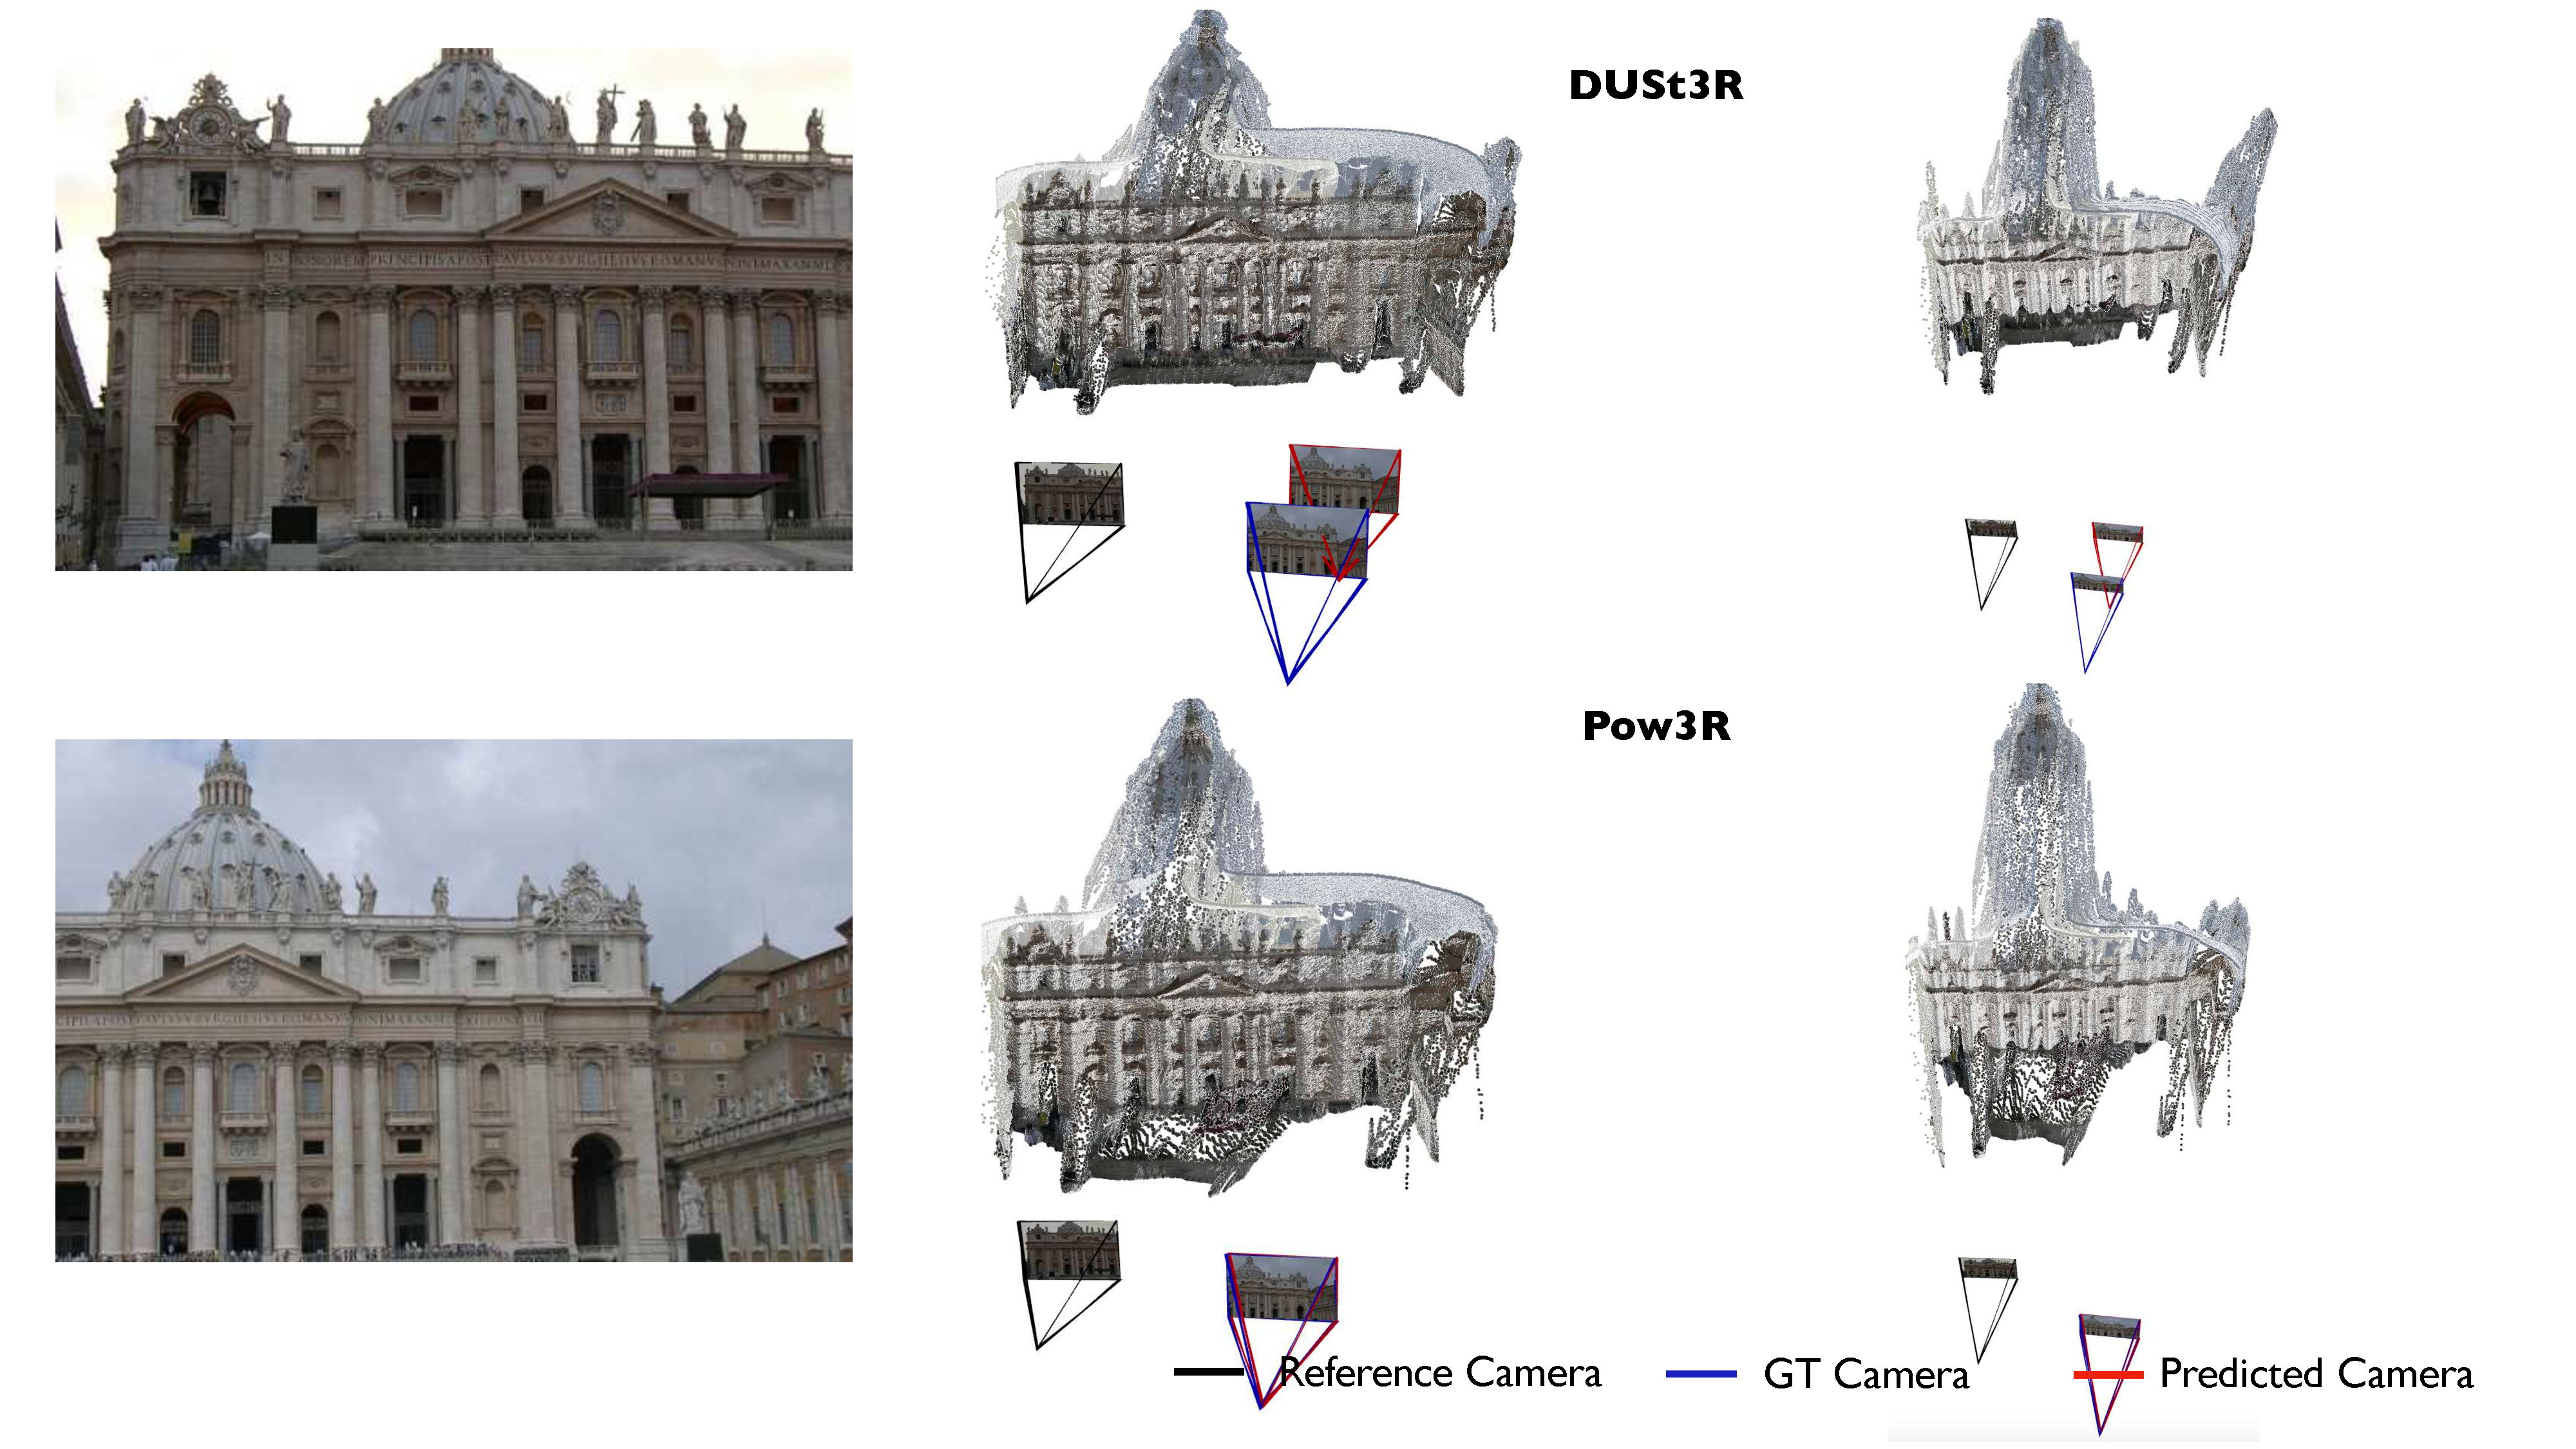
\includegraphics[width=\linewidth]{figures/supp/megadepth_figure2.pdf} \vspace{-0.5cm}
    \caption{\textbf{Qualitative Result on 3D reconstruction and camera estimation} on an outdoor scene from the Megadepth~\cite{li2018megadepth} dataset. We feed camera intrinsics, pose and 2048 sparse depths. \ours{} excels at reconstructing the depth of field and the camera locations, contrary to \duster{}.}
    \label{fig:qualitative_megadepth2}
\end{figure*}

\begin{figure*}
    \centering
    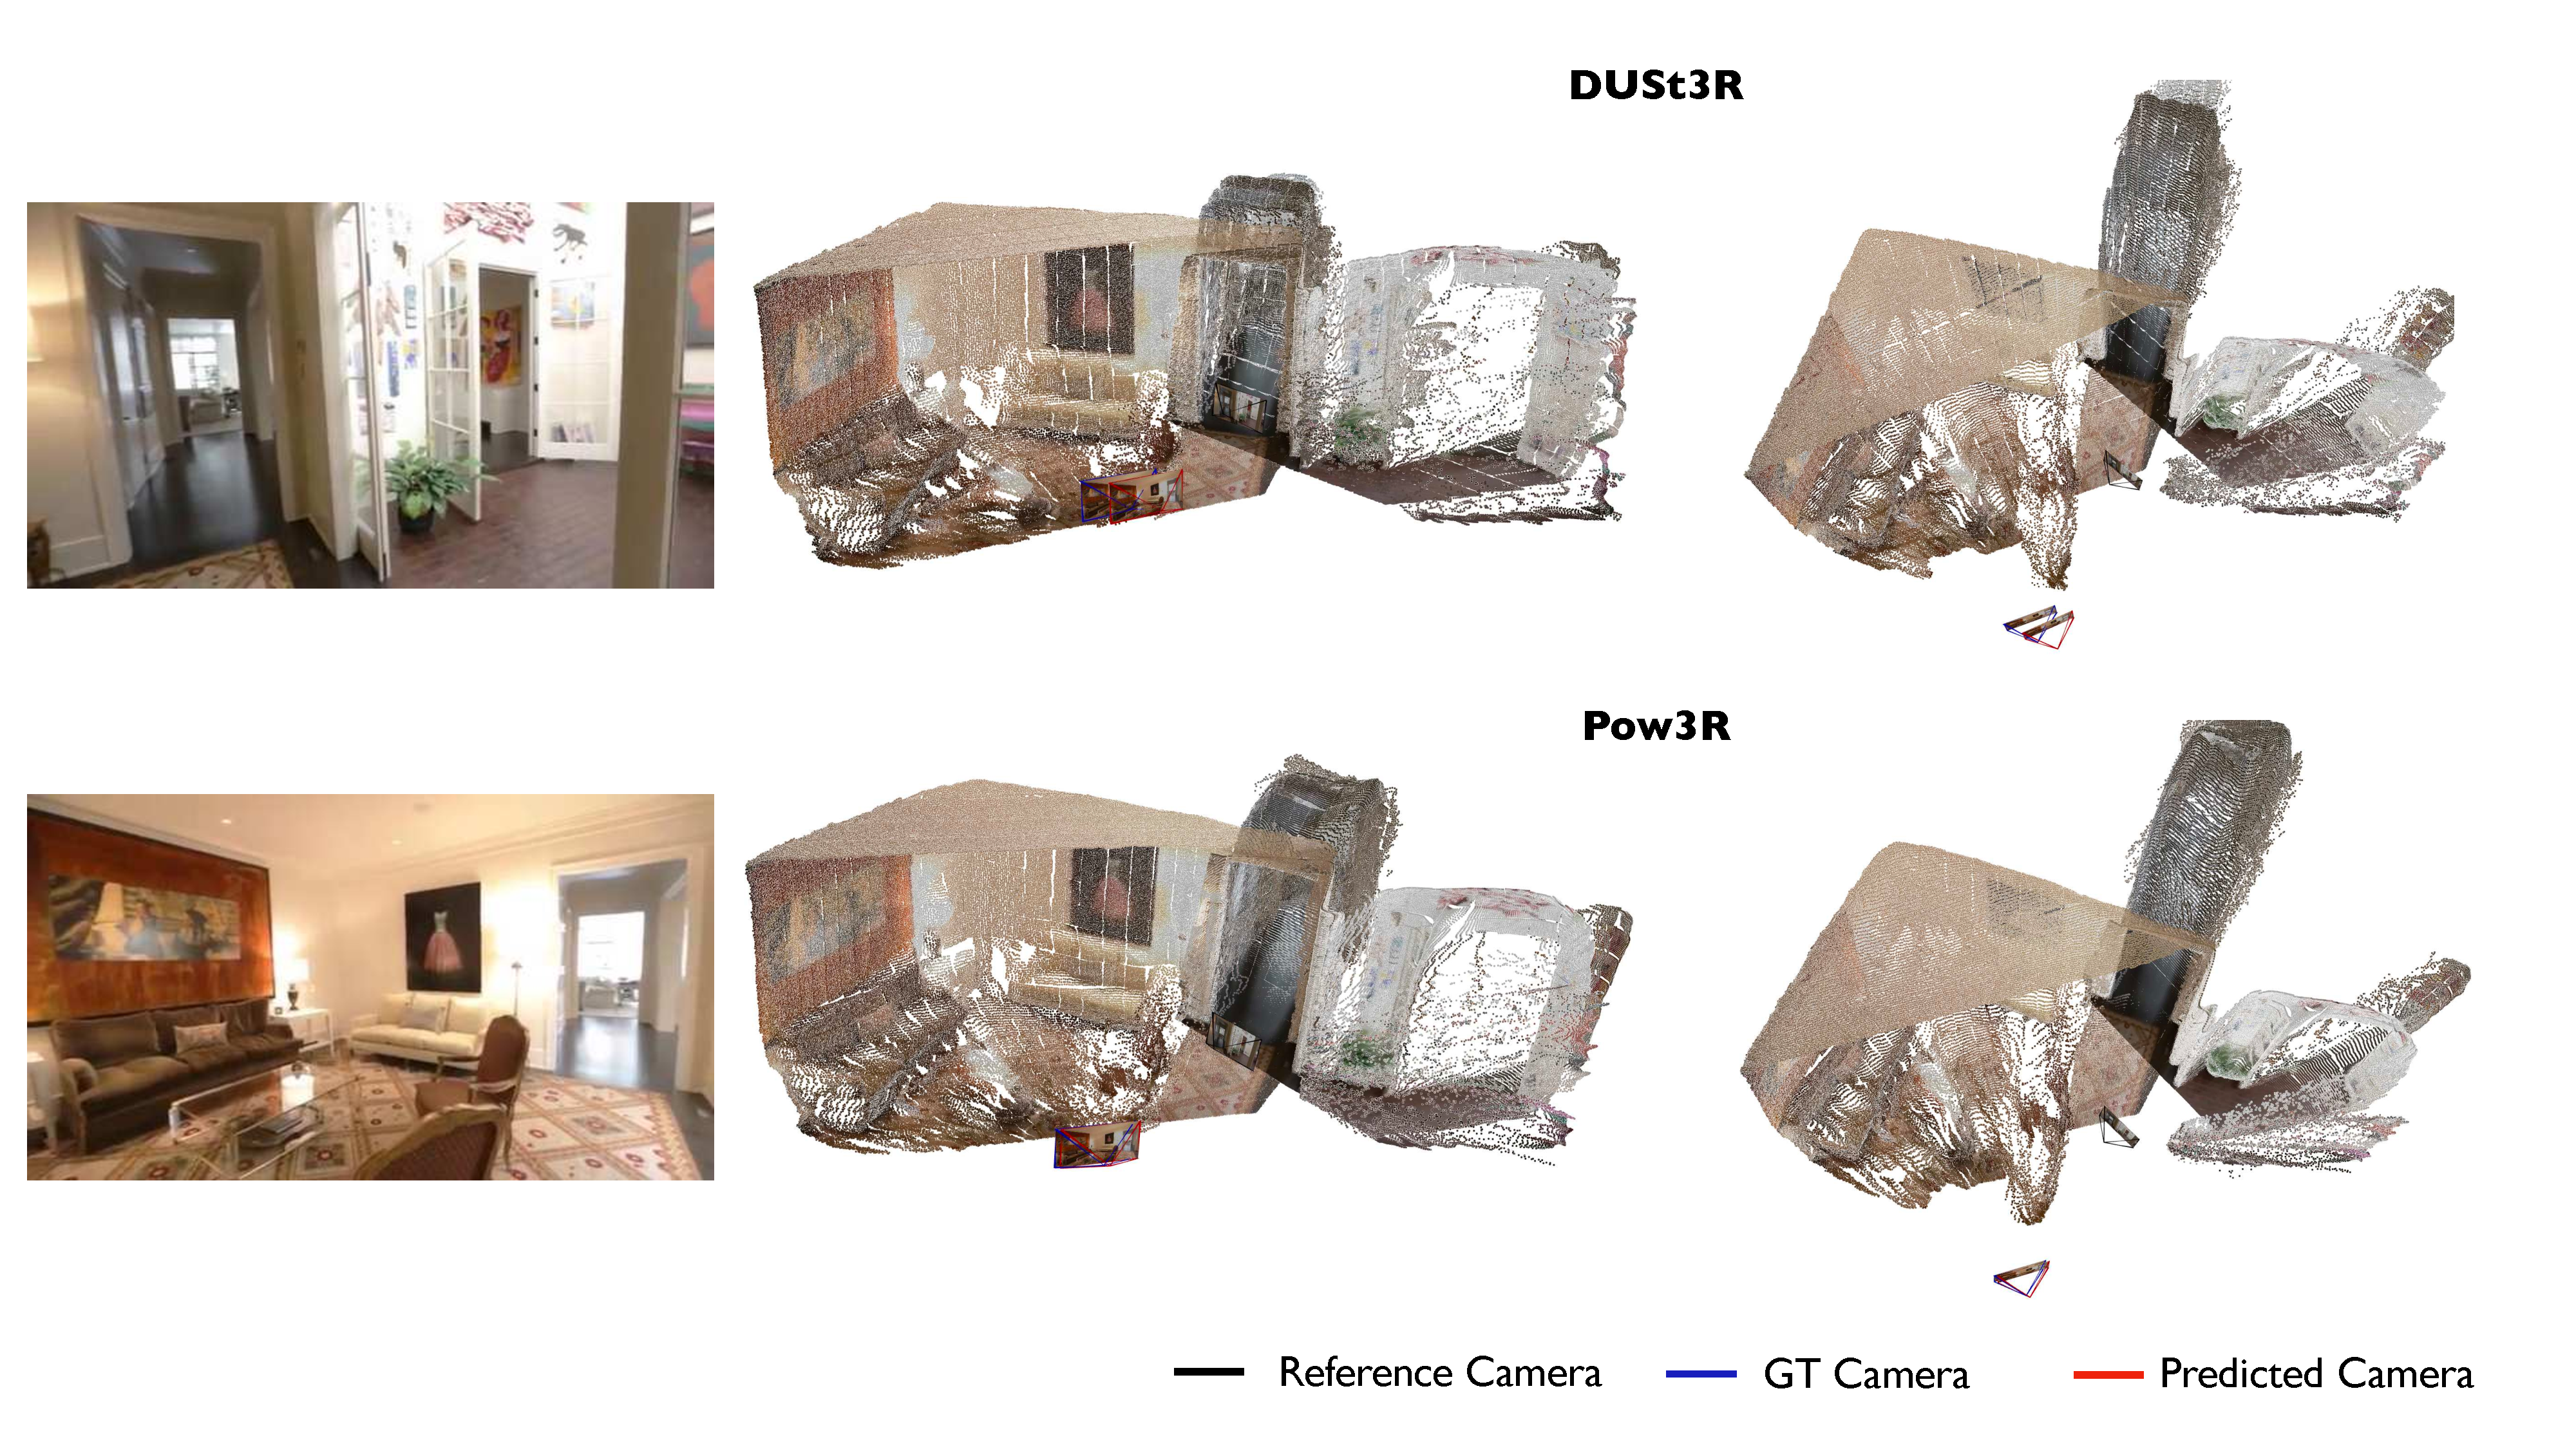
\includegraphics[width=\linewidth]{figures/supp/re10k_figure.pdf} \vspace{-0.8cm}
    \caption{\textbf{Qualitative Result on 3D reconstruction and camera estimation} on an indoor scene from RealEstate10K~\cite{realestate10K} dataset. In this evaluation, we only provide the camera intrinsics and extrinsic, as RealEstate10K dataset does not have point clouds or depthmaps. Both \ours{} and \duster{} produce faithful 3D reconstructions from two diverging viewpoints,  \ours{} demonstrates better performance at predicting camera locations than \duster{}.}
    \label{fig:qualitative_re10k}
\end{figure*}

\begin{figure*}
    \centering
    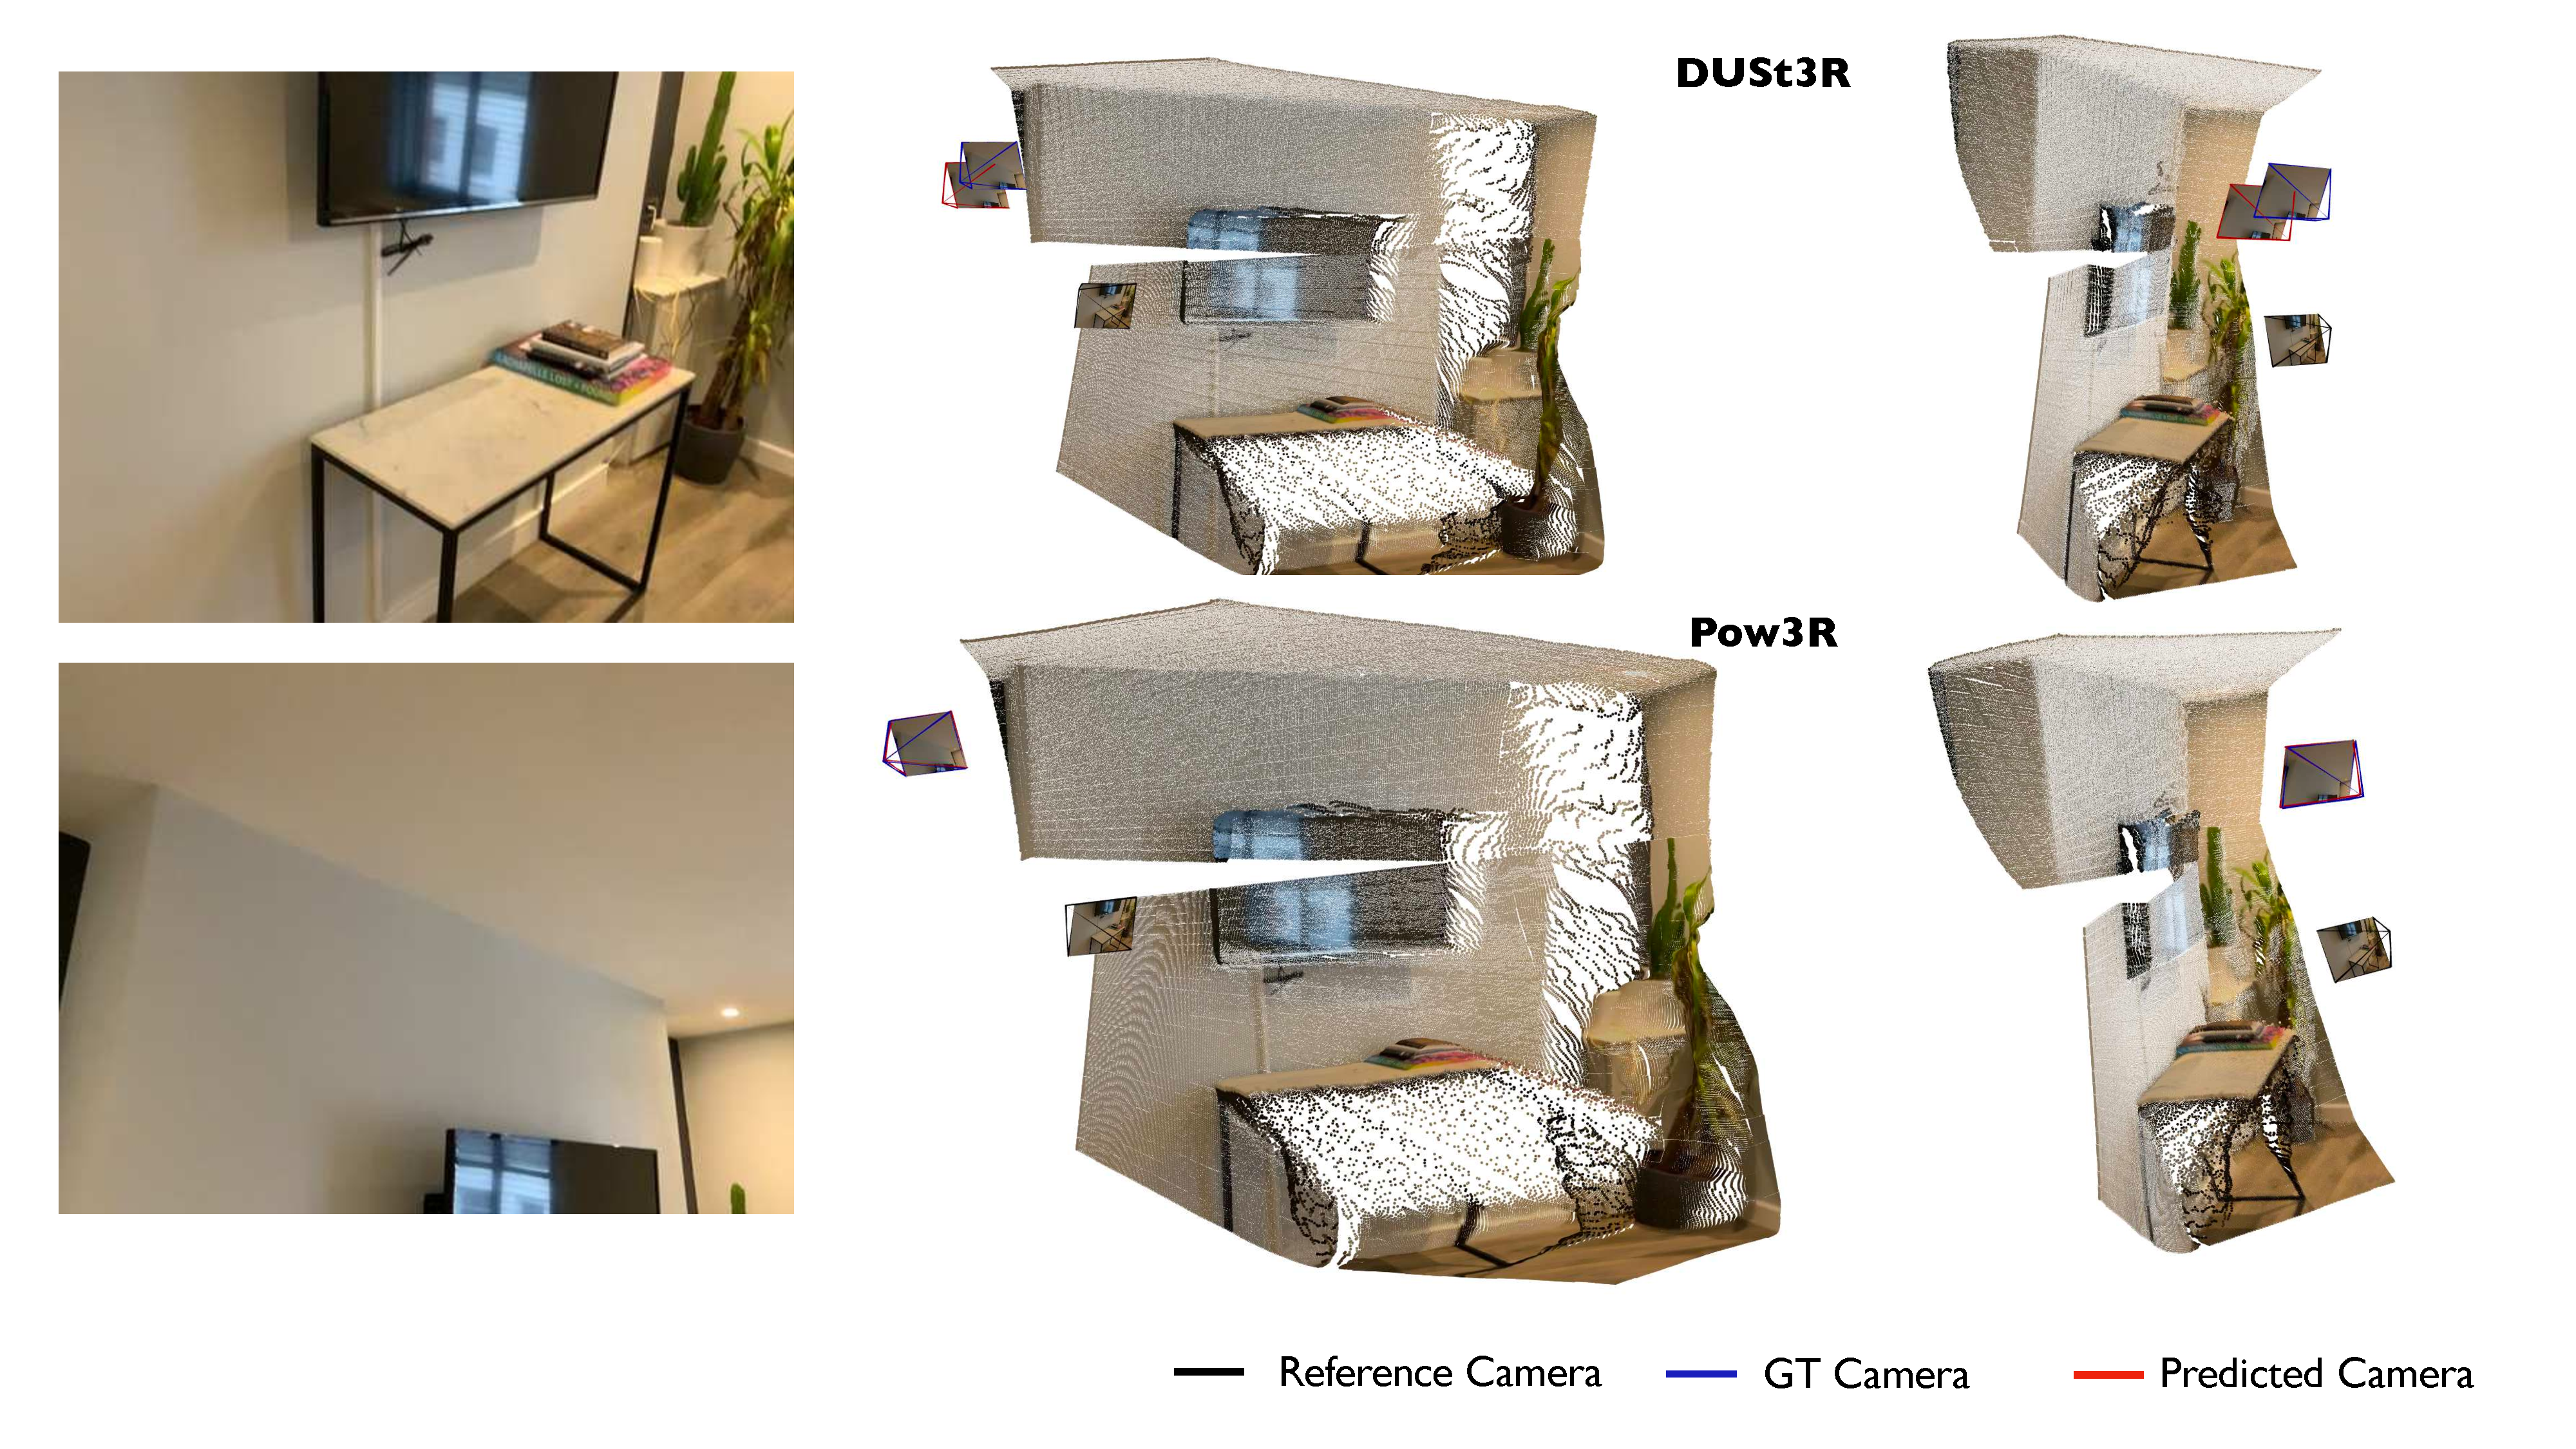
\includegraphics[width=\linewidth]{figures/supp/arkit_figure.pdf} \vspace{-0.8cm}
    \caption{\textbf{Qualitative Result on 3D reconstruction and camera estimation} on an indoor scene from ARKit~\cite{baruch2021arkitscenes} dataset. We provide to \ours{} camera intrinsics, pose and 2048 sparse depth points. Both \ours{} and \duster{} generate a reasonable 3D scene from two almost non-overlapping viewpoints, \ours{} providing more accurate camera locations than \duster{}.}
    \label{fig:qualitative_arkit}
\end{figure*}